\documentclass{article}
\usepackage{graphicx}
\usepackage[rightcaption]{sidecap}
\graphicspath{ {./billeder/} }
\usepackage{amsmath,amsfonts,stmaryrd,amssymb}
\usepackage[ruled]{algorithm2e}
\usepackage[framemethod=tikz]{mdframed}
\usepackage{parskip}
\usepackage{nameref}
\usepackage{booktabs}
\usepackage{tabularx}
\usepackage{geometry}
\geometry{
	paper=a4paper,
	top=2.5cm,
	bottom=3cm,
	left=2.5cm,
	right=2.5cm,
	headheight=14pt,
	footskip=1.5cm,
	headsep=1.2cm,
	%showframe, % Uncomment to show how the type block is set on the page
}

\usepackage[utf8]{inputenc}
\usepackage[T1]{fontenc}
\usepackage{XCharter}
\usepackage{graphicx}

\author {Jesper Toplund}
\title{Roadmap for komponenter}
\date{}

\begin{document}
\maketitle

\vspace{20 mm}
\begin{quote}
    \textit{}
\end{quote}

\section{Formål}
Det primære formål med rapporten er at opridse et roadmap for hvad vi bør fokusere på, hvis vi gerne vil opnå en sammenhængende, tidssvarende og vedligeholdbar arkitektur.

\section{Omfang}
Denne rapport er skrevet ud fra information i DR-systemkatalog og de betragtninger der er blevet gjort i forbindelse med arkitekturrapporten udarbejdet i samarbejde med Eksponent. Estimater og overslag, der er angivet i rapporten, er foretaget ud fra et kvalificeret bud på besvær og omkostninger og ikke ud fra en detaljeret analyse af hvert enkelt projekt. Mere præcise estimater vil være mulige for hvert delopgave, men er uden for scope af denne rapport.
 
Mere præcise estimater vil være mulige for hvert delopgave, men er uden for scope af denne rapport.

\section{Executive summary}
Arkitekturen i Web \& Apps bærer præg af at have vokset organisk frem. Når et forretningsproblem har vist sig, er en løsning på problemet lavet ud fra de for håndenværende ressourcer og kompetencer, uden hensyntagen til hvordan løsningen passer ind i resten af systemlandskabet. Det har resulteret i at vi i dag har mange eksempler på parallelle implementeringer, på systemer der ikke kan vedligeholdes, på ukendt aftagerlandskab og på fragmenteret infrastruktur.

% Hvad er formålet med at gennemgå disse skridt? Kan det opridses på forhånd?
De vigtigste skridt vi skal igennem er følgende:
\begin{itemize}
\item Design af gennemgående datamodel
\item Konsolidering af infrastruktur
\item Omskrivning af forældede produkter
    % Sikre et tilstrækkeligt fundament, eller at der ER et fundament?
\item Sikre DevOps fundament
\end{itemize}
Vi skulle gerne ende op med en arkitektur, hvor det er muligt at have styr på vores aftager-landskab. Vi skal også have mulighed for hurtig kommunikation imellem interne komponenter via sikret og afgrænset netværk. Det skal være muligt at teste komponenter individuelt og i et sammenhængende produktionslignende test setup.

Vi kan passende gå i gang med de lavt hængende frugter i form af at flytte de letteste kandidater over på pipeline, imens vi går i gang med de designtunge dele af opgaven (f.eks. design af fælles datamodel og redesign af relationssystem).

Det er svært at tids estimere præcist uden at grave dybere ned i detaljerne for de enkelte opgaver. Selve transformationen vil formentligt tage 2 år eller længere. Hvis vi i den tidsperiode stadig vil kunne varetage normale udviklingsopgaver, så bør vil allerede nu overveje at mande op i de forskellige teams.

\section{Forretningsbehov}


\subsection{Nyhedsapp}
Nyhedsappen har fungeret fint i 4 år og er i efteråret 2019 blevet vurderet af app bureauet Nodes som værende så godt optimeret som det er muligt baseret på den teknologi den er bygget på. Hvis nyhedsappen skal fortsætte med at være tidssvarende og blive ved med at give en god brugeroplevelse, så var det Nodes anbefaling at skifte over til en native applikation. Det vil sige at der skal udvikles en native IOS og en native Android version.

Hvis vi skal have en bedre brugeroplevelse eller markante udvidelser af nyhedsappen, så skal vi efter alt at dømme bygge appen helt op igen fra bunden af i en Native udgave. I den forbindelse vil det være meget relevant at vi også sikre datagrundlaget og platformen under appen, så vi kan få den bedst mulige brugeroplevelse.
Hermed vil det være relevant at sikre datamodel, event system og relations system er forberedt på denne udvikling.

\subsection{Drupal 7 pensioneres}
Drupal 7 (og Drupal 8) står over for End Of Life i november 2021. Inden da skal vi have taget stilling til hvordan vi skal fortsætte derfra.
Oprindeligt var Drupal hele vores udgivelses platform og det styrende system for alt indhold på DR.dk. I den rejse som DR.dk har været på de sidste par år, er flere og flere af Drupals oprindelige ansvarsområder blevet flyttet ud af Drupal og over i andre systemer. Dermed står vi med markant andre behov i forhold til CMS system end vi gjorde da vi oprindeligt valgte Drupal 7. Det er ikke nødvendigvis en direkte udskiftning af Drupal 7 med Drupal 9 der giver mest mening. 

For at sikre at vi kan tage det bedst mulige valg over for denne udskiftning skal vi sikre at vores Datamodel er på plads og vi har afdækket API og event behov i forhold til redaktør grænsefladen og artikel database. 

\subsection{Relations system}
Garnnøgle og TAG system har af flere omgange været oppe og vende som problematiske systemer. Garnnøgle er i en kritisk tilstand hvor det er stort set umuligt at vedligeholde eller videreudvikle på. Ud over Garnnøgle og Tag, så er der også en række andre systemer der varetager relationshåndtering i større eller mindre omfang.

Da relationssystemer både har stor forretningsmæssig potentiale og er i kritisk vedligeholdelsestilstand, så er det et oplagt område at prioritere i vores systemgennemgang.

\subsection{Udgivelseshastighed}

En stor del af den kompleksitet der er i vores platform i dag er på grund af afhængighederne imellem systemerne. Hver gang der er forbindelse mellem to systemer hvor det afhænger af en brugerhandling eller et push af informationer fra et system til et andet system, så er der mulighed for forbedringer både i form af reaktionstid men også i form af systemkompleksitet ved at vende afhængighederne om og lade alle systemer udstille generaliserede APIer og lade systemer udgive og abonnere på events i forbindelse med opdateringer.

I dag, når en artikel udgives i Drupal, så skabes der et event, som opfanges af mimer og bruges til at igangsætte indekseringen.
Hvis vi raffinerer den løsning og benytter et fornuftigt besked framework, så kan den samme besked benyttes til at igangsætte alle de andre tjenester rundt omkring, som også skal være på plads for at en artikel er søgbar på dr.dk.

Disse events og lignende events fra andre dele af systemet kan benyttes til at lade opdateringerne propagere ud til alle dele af systemet, inklusiv at opdatere cache lag, forside lister, personaliserings søgninger, markering af Breaking artikler, push af notifikationer til Nyhedsapp  osv. 

Et publiceringsevent vil dermed selv kunne triggere indeksering fra Cxense, opdatering af cache, opdatering af Garnnøgle og lignende. Det vil effektivt få ventetiden på opdatering ned i nærheden af hvad de enkelte systemer kan præstere.
Ligeledes vil en eventbaseret arkitektur sikre at vi ikke behøver at pushe fra et system til et andet, men kan nøjes med at udstille APIer så et system ikke behøver at kende sine aftagere, blot at overholde den aftalte datakontrakt.


\section{Vision}
Web og Apps har i de sidste år gennemgået en betydelig omstrukturering af deres miljøer og services. Det landskab vi står med i dag er i langt højere grad forberedt på at håndtere de skiftende krav til danskernes medieforbrug. Der er blevet foretaget en række gode valg i opdeling af ansvar og løsere kobling imellem systemer. Denne transformation er dog foregået med begrænset koordination ud fra de behov der opstod undervejs. 

Det efterlader os i dag med en arkitektur af en noget organisk karakter, hvor mange design valg er taget med et specifikt produkt for øje i stedet for at gennemtænke hvordan platformen i sin helhed kan få glæde af og inkorporere en given funktionalitet.

Det er svært at spå om præcist hvad fremtiden vil bringe af udfordringer og muligheder, det er dog muligt at spå om hvilken funktionaliteter der vil gøre det muligt for os at møde den.  

\subsection{Cloud strategi}
DR har i årevis gået efter en Cloud strategi. Den har vi i DR.dk efterlevet efter bedste evne i den enkelte teams. Resultatet heraf er at der i hvert team er blevet taget en række valg om pipeline, hosting og platform.
De enkelte teams løsning af problemet har dermed resulteret i 4 forskellige skyer og release processer. Den manglende ensretning betyder at der er noget spild arbejde i form af at vedligeholde de 4 forskellige byg og deploy pipelines men især også at der er nogle uhensigtsmæssige afhængigheder på tværs af disse skyer. 
Alle 4 skyer skal i spil når en ny artikel skal udgives og et udfald hos hvilken som helst af de 4 udbydere betyder at et led i kæden knækker og dermed at artikler ikke kan udkomme. Vi udnytter dermed ikke de fordele der kan være ved at have vores hosting spredt ud, men vi får ulemperne ved det.
\begin{itemize}
\item Offentligt tilgængelige endpoints der kun burde benyttes til intern kommunikation
\item Betaling for trafik mellem sky udbydere
\item Manglende ensretning af den underliggende platform
\item Ekstra latenstid imellem komponenter 
\end{itemize}
Vi bør konsolidere vores cloud strategi til at benytte den samme udbyder på tværs af teams og gerne også en fælles pipeline. Dermed vil vi opnå både en ensartet release og deploy process og vi vil samtidigt fælles kunne høste de forbedringer som et fælles miljø vil kunne tilbyde.


\subsection{Antallet af systemer der aftager artikler vil efter alt at dømme stige}
Vi bør derfor sørge for at adskille visningslag fra artikel lag i videst muligt omfang og sikre en konsistent datastruktur for artikeldata. Hvis vi får etableret en gennemgribende datamodel, så vil den samme platform kunne levere artikel data til hvilket som helst medie (web, IOS / Android, nyhedsbreve, RSS feeds, TTV osv.) der måtte forbruge det og vi vil stadig være i stand til at give en rimeligt konsistent oplevelse på tværs af medier.

Vores mål arkitektur bør i videst muligt omfang være forberedt på at vi ikke nødvendigvis kender aftager landskabet i morgen, så jo bedre vi er i stand til at udstille vores indholdsdata i en veldefineret format på så mange niveauer som muligt, jo bedre vil vi være i stand til at imødekomme ønskerne fra morgendagens aftagere, om det så er interne eller eksterne aftagere.


\subsection{Event system}
Vi bør anvende et Eventsystem med et fornuftig interface, respektable service kontrakter og som kan sikre hurtig besked håndtering i mellem systemerne.

For at holde os til en enkelt cloud udbyder og ikke eksponere os for øget responstider og risiko, så bør vi kikke på om vi kan benytte googles "Cloud pub/sub" eller om der er et andet system der vil passe bedre.


\subsection{Behovet for personalisering vil blive endnu højere}
Både forbrugere og redaktører stiller større og større krav til at vi kan vise de mest relevante artikler for en given bruger. For at imødekomme dette bliver vi nød til at få kikket nærmere på personalisering og integrationerne med de eksterne systemer vi benytter til dette.

Cxense er et godt eksempel på et kraftfuldt eksternt system, som vi ikke benytter til fulde endnu. Vi benytter f.eks. ikke de APIer Cxense  udstiller til at sikre rettidig indeksering af publicerede sider, lige som vi ikke relaterer brugerkonti med Cxense brugerID i forbindelse med udsendelse af nyhedsbreve.


\subsection{Afdækning af trends i forbrugsmønstre vil blive mere og mere relevant}
Det er vigtigt at vi holder for øje at det bør være muligt at holde styr hos forbrugsmønsteret hos vores brugere. Jo bedre vi kan spore forbrugsmønsteret på tværs af platformen, jo bedre vil vi være i stand til at imødekomme fremtidens behov og dokumentere i hvilket omfang vi opfylder de forventninger vi har til platformen.
Vi skal med GDPR reglementet for øje have sikret at vi opfanger det relevante data der skal til for at kunne gøre vores platform så brugervenlig som mulig.


\subsection{Større behov for at kunne linke på tværs af platforme}
Det har længe været et ønske at kunne binde Radio, TV og Nyhedsartikler tættere sammen end nu. Især set ud fra personaliserings synspunkt kan det være meget relevant at kunne relatere nyhedsartikler med enten on demand radio eller video segmenter.
Hvad end behovet vil være, så bør vi være sikre på at vi er forberedt på at understøtte disse relationer, både i form af adfærdsanalyser på tværs af platforme og også i form af relationssystemer der kan linke radio, video og artikler.


\section{Generelt forarbejde}
\subsection{Indholdsdatamodel}
Noget af det vigtigste for at få arkitekturen til at hænge sammen, er at vi etablerer en generel og gennemgående datamodel, som kan være med til at sikre at alle vores komponenter kan kommunikere på tværs. Det er et vigtigt stykke forarbejde, som både bidrager til muligheden for at rydde op i den nuværende hårknude-arkitektur, og gør det muligt at sikre at nyudviklede komponenter kan benyttes på tværs. Det kommer til at kræve en del arbejde at få etableret denne datamodel og derefter at få de forskellige systemer tilpasset til denne datamodel.

% Hvad er argumentet for at læne sig op af Steffis tilgang? Djævlens advokat ville indvende,
% at Steffi ikke udstiller en datamodel, men en liste af attributter som aftagere kan vælge ud fra?
% NB: Jeg er ikke uenig, men savner argumentation og ligeledes klarhed over hvilke dele fra Steffi,
% der bør tjene til inspiration. Min frygt er at man *benytter Steffis tilgang, og dermed får
% en datamodel som er en visningsmodel, altså hvilke felter der skal vises i frontend.
Det anbefales at vi starter med at udarbejde en så dækkende model som muligt. Her kan vi passende tage udgangspunkt i den datamodel der allerede benyttes af Steffi og afdække hvorvidt den dækker de behov vi kan forudse. Dermed får vi et centralt udgangspunkt som, når det bredes ud, kan bruges som samlingspunkt om vores content aggregation service. 

Datamodellen skal ikke nødvendigvis implementeres på tværs af hele dr.dk fra starten af, men det vil være til stor gavn hvis vi kan arbejde os i retning af en fælles datamodel i alle fremtidige større ændringer af systemerne,
samt i al større nyudvikling.
Udarbejdelse af datamodellen bør ske inden næste store ændring i et af de centrale indholdsbærende datalag (Mimer, Steffi, Hydra, Nyhedsapp eller lignende).

    \textit{TODO: evt et estimat}


\subsection{URN / URL}
Vi bør i forbindelse med arbejdet på datamodellen også kikke på at få etableret en URN / URL der unikt kan identificere et hvilket som helst stykke indhold på tværs af systemlandskabet. Denne URN skal være i stand til unikt og konsistent kunne identificere en artikel, en relationsliste, et billede eller hvad som helst andet. Det bør ud fra URN alene være muligt at slå indhold op uden at man nødvendigvis kender det underliggende systemlandskab. Det vil gøre det muligt at have meget løst koblede systemer.
% Kan det uddybes hvad problemstillingen er, og hvilke fordele vi kan opnå
% ved at udrulle/ensrette URN/URL?
    \textit{TODO: Mere fyld!}

\subsection{Underliggende infrastruktur}
Alt indhold på dr.dk serves i dag igennem Akamai CDN. Akamai fungerer som Content Delivery Network, DDOS-beskyttelse og cache-lag. I tilfælde af udfald på dr.dk er cache hos Akamai sat
til at blive ved med at servere nuværende data, indhtil vi igen er i stand til at besvare på forespørgsler på dr.dk. Det betyder at forlængede svartider eller korte nedbrud ikke nødvendigvis bliver bemærket hos slutbrugeren.

Infrastrukturen som i dag driver dr.dk har et par fordele men også en række ulemper. Hvert team har valgt hosting og teknologi ud fra hvad de kender til og deres lokale ønsker om funktionalitet. Det betyder at vi i dag har dele af dr.dk hostet på fem forskellige cloud platforme,

\begin{itemize}
    \item AWS (eks. Drupal)
    \item Azure (dr.dk-forside, Nyhedsapp-backend)
    \item DR-byens datacenter (primært legacy-produkter)
    \item Google Cloud (produkter på DR Pipeline)
    \item Heroku (eks. Steffi, Hydra)
\end{itemize}

For at en artikel kan udkomme på dr.dk-forsiden og i Nyhedsapp skal der udveksles data på tværs af alle fem skyer.

Kommunikationsudfald eller nedbrud hos en af cloud-udbyderne vil i de fleste tilfælde betyde, at vi ikke kan udkomme med nye artikler. Der er ingen driftsmæssig fordel ved at vi har baseret vores infrastruktur på fem forskellige skyer, da udgivelse af en artikel vil fejle lige meget hvilket led i kæden der knækker. 

\subsection{Parallelliseret og distribueret system}
DR har i kraft af Public Service-kontrakten med staten, en forpligtigelse til at kunne udkomme med nyheder og varslinger hele tiden og med kort varsel.
Det stiller selvfølgeligt krav til vores systemers oppetid. Jo tættere koblet et system er, jo mere sårbar er det over for nedbrud i kæden af de systemer, det er koblet til.
De systemer vi selv hoster og drifter, bør sikres i det omfang det er muligt. Jeg vil foreslå at vi kikker grundigt på et parallelt sky-setup, så vi f.eks. har en primær region (europe-west2) hvor der er veldefinerede skaleringsregler og etableret overvågning.
Vi kan samtidigt have en sekundær sky sat op i en anden region (f.eks. europe-west4) som er skaleret helt i bund og ingen trafik varetager.
Ved nedbrud i den primære region kan vi skifte til den sekundære og lade den skalere op.

    \textit{TODO: Grovestimat af fordele / ulemper ved dette}


\subsection{DevOps-kulturen styrkes}
Den primære fokus i DevOps kulturen er et forsøg på at gøre op med de forskelle der er imellem en udviklingsafdeling og en driftsafdeling. Dette er primært ud fra anerkendelsen af at udviklerne af et stykke software formentligt også er dem der bedst er i stand til at finde og rette fejl i deres software.

Et vigtigt element i dette er at det skal være muligt for udviklerne at teste i et produktionslignende miljø og at kunne deploye en rettelse til produktion med god antagelse af at det ikke har en negativ impact på resten af infrastrukturen. 

Det er her relevant at kikke nærmere på elementer fra CI/CD kulturen (Continuous Integration / Continuous Deployment). Standardiseret byg pipeline, statisk kodeanalyse, afvikling af unittests og automatiseret deploy til test miljø og relateret tiltag vil være med til at finde fejl og mangler så tidligt som muligt, så releases til produktion kan ske både trygt og hurtigt.

\subsubsection{Ensretning af pipeline}
De pipelines der i dag benyttes på tværs af web og apps er ret optimeret i forhold til de enkelte teams og deres release process. Hvis vi går fra en specialiseret til en generel pipeline vil de enkelte teams releaseprocess skulle tilrettes markant for blot at opnå den samme funktionalitet som i dag. Der vil dog være store fordele der kan høstes hvis pipelinen benyttes af flere teams. 
\begin{itemize}
\item Fælles værktøjer
\item Central udvikling af værktøjer
\item Standardiserede værktøjer til statisk kodeanalyse
\item Standardiseret deployment værktøj
\item Fælles repository af deployet kode
\end{itemize}


Det vil ligeledes give den fordel at det vil være lettere for udviklerne at aflaste hinanden på tværs af teams, da værktøjer og standarder på pipelinen er fælles, så det kun er kodeforskelle der er behov for at sætte sig ind i.
 
\subsubsection{Testmiljøer}
Ideelt set skal det være muligt at deploye et komplet miljø til enten test eller produktion fra et centralt sted. Det må meget gerne være muligt at have et aktivt produktionssystem, et inaktivt produktionssystem, et aktivt test system og mulighed for deploy af dedikerede testsystemer. 

\begin{itemize}
    \item fast fuld funktionibelt testsystem (staging).
    \item mulighed for deploy af nyt miljø med nødvendige komponenter.
\end{itemize}


\subsubsection{Fælles overvågning}
Udviklerne i de enkelte teams er specialister i deres egne systemer og er som sådan, de bedst egnede til at fejlfinde og vedligeholde deres systemer. Det betyder dog ikke at udviklerne er de bedst egnede til at overvåge og fejlfinde i infrastrukturen som systemerne kører på. Ideelt skal vores systemer køre på en fælles platform, som der kan overvåges centralt.
Ideelt set burde platformen overvåges centralt, med veldefinerede alarmer på alle miljøer. I tilfælde af nedbrud på et miljø bør overvågningen have en drejebog på hvilke skridt der kan foretages for at afhjælpe problemerne.
For at opnå det er der behov for følgende:
\begin{itemize}
\item Konsolidering af driftsmiljøer.
\item Velbeskrevne overvågningsparametre.
\item Velbeskrevet drejebog for afhjælpning af problemer.
\item Velbeskrevne eskaleringsmuligheder af problemer.
\end{itemize}

Udviklerne i de enkelte teams har ansvaret for udvikling, test og vedligeholdelse af deres systemer. Udviklerne skal ligeledes sørge for at der opsættes overvågningspunkter, så der kan rapporteres systemstatus til overvågningen samt drejebøger for hvordan almindelige fejl kan afhjælpes.
DevOps-afdelingen skal stå for udvikling af de nødvendige værktøjer og skal have det formelle ejerskab af infrastrukturen. Hvis der er nedbrud på netværk, hosting eller andre infrastrukturkomponenter, så skal dette løses af ejeren af infrastrukturen.

Overvågningen kan varetages af Infra-afdelingen. Denne overvågning skal være af både infrastruktur og overvågningspunkter der leveres af udviklerne i de enkelte udviklingsteams. Da hverken DevOps eller de enkelte udviklingsteams har døgnbemanding, er Infra reelt eneste mulighed for at afhjælpe problemer på platformen uden for normal arbejdstid.

%* DevOps tankegangen er et strålende bud på en løsning af 3 delingen mellem infrastruktur, drift og udvikling.
%* Devops skal styrkes i de enkelte udviklings teams.
%	De skal kunne lave hyppige releases.
%	De skal kunne lave sikre releases.
%	De skal kunne overvåge deres applikationer.
%	De skal kunne fejlfinde i deres applikationer på tværs af hele platformen.
%Centraliseret overvågning af infrastrukturen.
%	De enkelte teams i Web og apps skal ikke være ansvarlige for overvågning af hele infrastrukturen.
%	Teams skal kunne fejlfinde i egne applikationer på tværs af hele platformen.

%TODO. Dette er nok det vigtigste afsnit. Her skal skrives MEGET


\section{Analyse af komponenter}

\subsection{Akamai}
\begin{figure}[h]
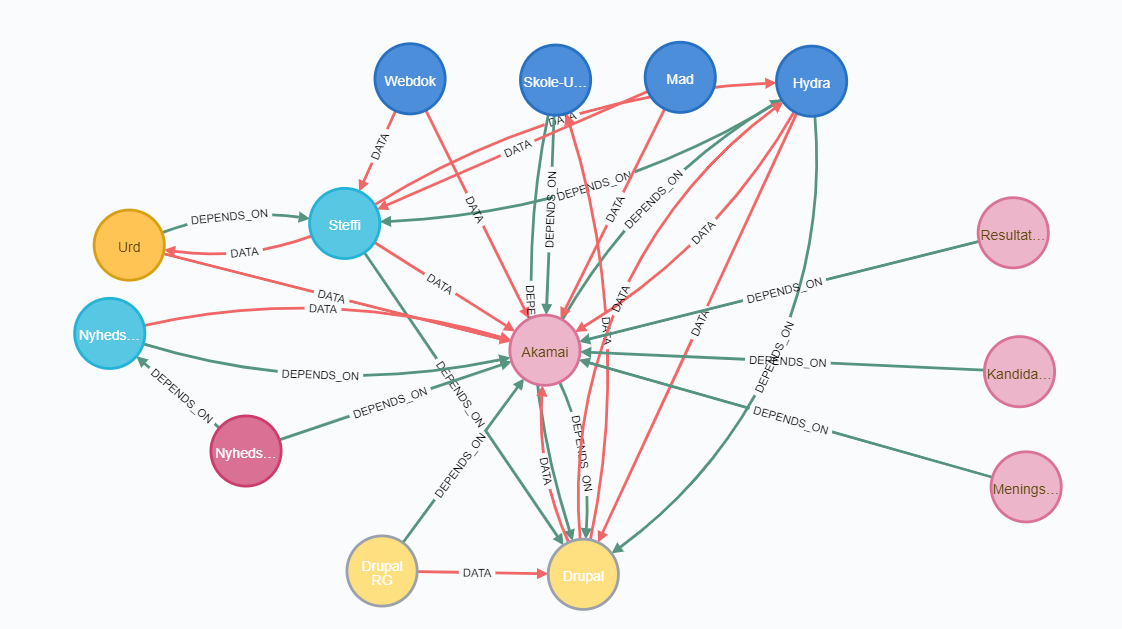
\includegraphics[width=300pt]{Akamai.PNG}
\caption{MATCH (x\{name:'Akamai'\})- -(y) RETURN x,y}
\end{figure}
\subsubsection{Kort beskrivelse}
Akamai benyttes som det primære CDN (Content delivery Network). 
Det er dermed ikke et produkt som er udviklet hverken af eller for DR, 
men et produkt som vi er afhængige af. 
\subsubsection{Anbefalet handling}
Akamai som CDN udfylder fint de behov som DR har. 
Vi kan med fordel kikke på om vi benytter fornuftige cache timeouts eller om vores hjemmeside er struktureret til at få mest muligt ud af CDN.

\subsubsection{Overslag}
Indgår ikke som sådan i roadmap.


\subsection{Hydra}
\begin{figure}[h]
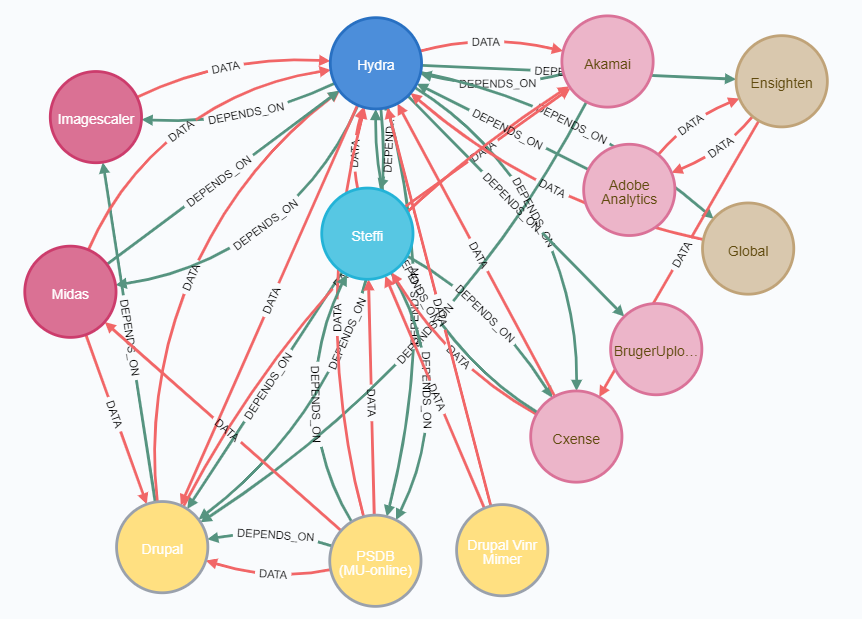
\includegraphics[width=300pt]{Hydra.PNG}
\caption{MATCH (x\{name:'Hydra'\})- -(y) RETURN x,y}
\end{figure}
\subsubsection{Kort beskrivelse}
Web-frontend, der varetager indholdsvisning for artikler og forsider. Anvender Drupal-visning til sider, der endnu ikke understøttes af Hydra.
Ovenstående figur viser at der er et højt antal afhængigheder til mange systemer. Det skal undersøges nærmere om de alle er aktuelle.
\subsubsection{Anbefalet handling}
Hydra er beskrevet som at den direkte henter data fra og sender data til Drupal. Er det korrekt, så springer den flere lag over i referencearkitekturen.
Hydra burde kun afhænge af platform utilities, platform services, product services eller content aggregation.
% TODO Verificer at alle de beskrevne afhængigheder også er aktuelle afhængigheder.
\subsubsection{Overslag}
Afklaring nødvendigt før det kan estimeres.


\subsection{Steffi}
\begin{figure}[h]
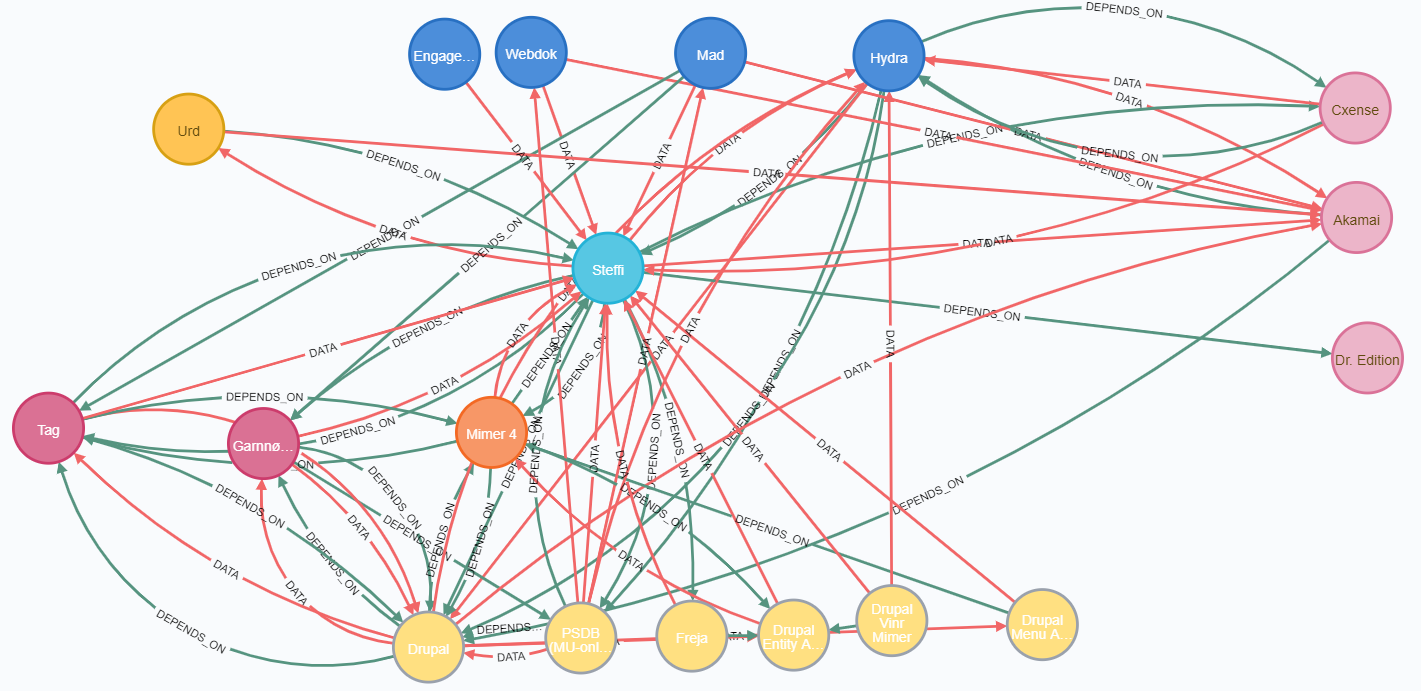
\includegraphics[width=300pt]{Steffi.PNG}
\caption{MATCH (x\{name:'Steffi'\})- -(y) RETURN x,y}
\end{figure}
\subsubsection{Kort beskrivelse}
Forespørgselslag, der tilbyder GraphQL-grænseflader til frontendapplikationer.
Benytter Content aggregering.



\subsection{Talentholdet}
\begin{figure}[h]
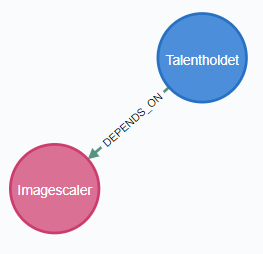
\includegraphics[width=80pt]{Talentholdet.PNG}
\caption{MATCH (x\{name:'Talentholdet'\})- -(y) RETURN x,y}
\end{figure}
\subsubsection{Kort beskrivelse}
Talentholdet er en rekrutteringsplatform for nye talenter til DR. Talentholdet har sin egen database hvori den gemmer personidentificerbar data i krypteret form. Talentholdet afhænger af Imagescaler
\subsubsection{Anbefalet handling}
Talentholdet udfører en mindre opgave som det er muligt at diskutere værdien af. Vi bør få afklaret med forretningen om vi eventuelt kan pensionere programmet. Der er en del kodegæld i programmet og GDPR-afledte sletninger er en manuel process.
Prioriteten af Talentholdet er dog ret lav, så den manuelle process kan tolereres.


\subsection{Elements}
\begin{figure}[h]
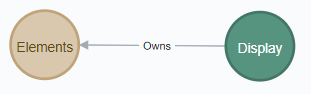
\includegraphics[width=120pt]{Elements.PNG}
\caption{MATCH (x\{name:'Elements'\})- -(y) RETURN x,y}
\end{figure}
\subsubsection{Kort beskrivelse}
Elements er DR's centrale komponentbibliotek, som består af frontendkomponenter. Elements er kodet i React. Elements benyttes af en række af vores frontend-produkter, men ikke alle.
\subsubsection{Anbefalet handling}
Elements benyttes af en række af vores frontend-produkter og passer fint ind i vores referencearkitektur.


\subsection{Webdok}
\begin{figure}[h]
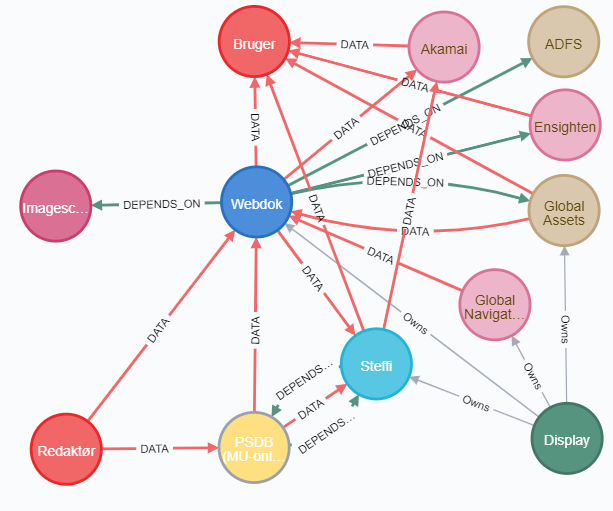
\includegraphics[width=180pt]{Webdok.PNG}
\caption{MATCH (x\{name:'Webdok'\})- -(y) RETURN x,y}
\end{figure}
\subsubsection{Kort beskrivelse}
CMS og præsentation af featureartikler i særformater.	
Præsentationslag (Node.js) trækker data fra API (Node.js). Redaktørgrænseflade er bygget ind i præsentationslaget.
\subsubsection{Anbefalet handling}
Hvordan Webdok er flettet ind i vores nuværende arkitektur skal undersøges nærmere. Dokumentationen som den står nu giver et lidt mudret billede
% TODO
\subsubsection{Overslag}
Ukendt.


\subsection{Skole-Undervisning}
\begin{figure}[h]
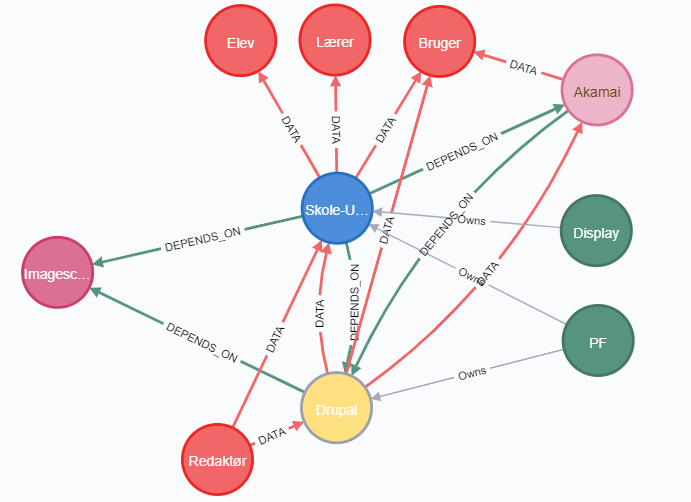
\includegraphics[width=80pt]{Skole-Undervisning.PNG}
\caption{MATCH (x\{name:'Skole-Undervisning'\})- -(y) RETURN x,y}
\end{figure}
\subsubsection{Kort beskrivelse}
Skole og Undervisning er et site, der formidler undervisningsforløb og undervisningsmateriale til Skoler.  Sitet er opbygget i Drupal, men har en række specialløsninger konstrueret for at kunne samle temaer og autogenerere faktabokse etc. 
\subsubsection{Anbefalet handling}
Skole-Undervisning passer ikke ind i referencearkitekturen, idet den udgør sin helt egen silo og udstiller data direkte til slutbrugere via Akamai. 
Afhængigt af levetiden for projektet (Gartners TIME-model) skal vi overveje hvad vi gør ved projektet.


\subsection{Mad}
\begin{figure}[h]
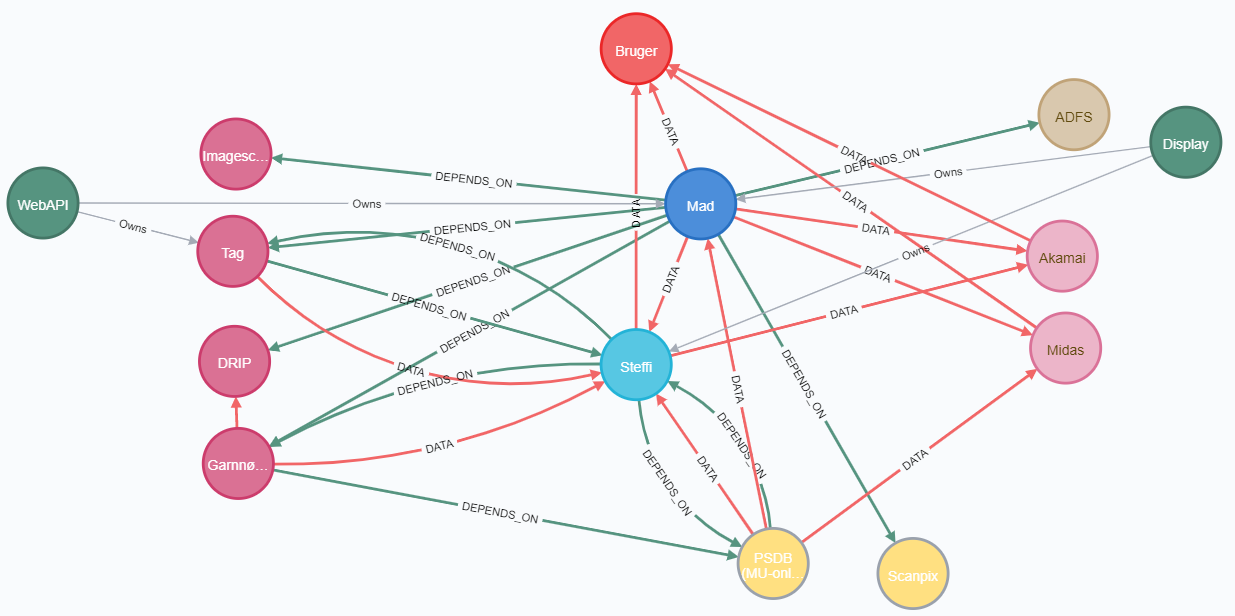
\includegraphics[width=240pt]{Mad.PNG}
\caption{MATCH (x\{name:'Mad'\})- -(y) RETURN x,y}
\end{figure}
\subsubsection{Kort beskrivelse}
Mad er en applikation, der håndterer opskrifter, artikler og opskriftssamlinger. Mad er bygget som Headless Drupal med egen RG til opskrifter. Artikler publiceres gennem Drupal. 
\subsubsection{Anbefalet handling}
Mad passer ikke helt ind i referencearkitekturen som beskrevet. Om det er en mangel i dokumentationen eller i arkitekturen skal undersøges. (hvorfor tilgår Steffi Mad direkte og ikke igennem f.eks. Mimer?)


\subsection{Nyhedsapp-Frontend}
\begin{figure}[h]
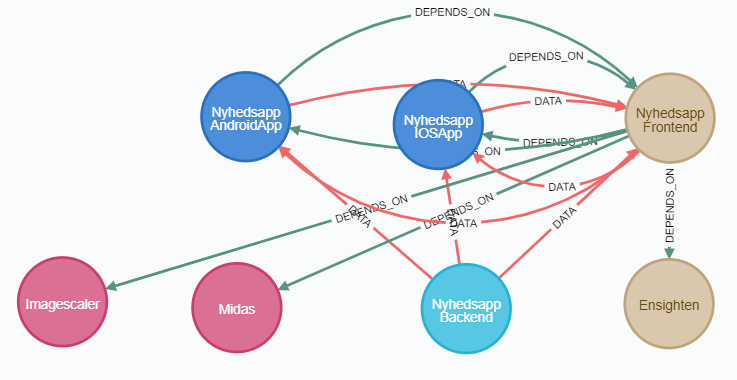
\includegraphics[width=160pt]{Nyhedsapp-Frontend.PNG}
\caption{MATCH (x\{name:'Nyhedsapp Frontend'\})- -(y) RETURN x,y}
\end{figure}
\subsubsection{Kort beskrivelse}
Præsentationslag for indhold i Nyhedsapp, således at visningen mellem iOS og Android er homogen, samt har lignende homogenitet til visningen på DR.dk
Nyhedsapp-Frontend er ikke en selvstændig applikation, men et delt kodelag der anvendes af iOS- og Android-udgaverne af Nyhedsapp. 
\subsubsection{Anbefalet handling}
Nyhedsapp-Frontend eksisterer kun i kraft af den aktuelle implementering af Nyhedsappen. Hvis Nyhedsappen skal opdateres eller udskiftes vil Nyhedsapp-Frontend også skulle opdateres eller skiftes.


\subsection{Nyhedsapp-iOS}
\begin{figure}[h]
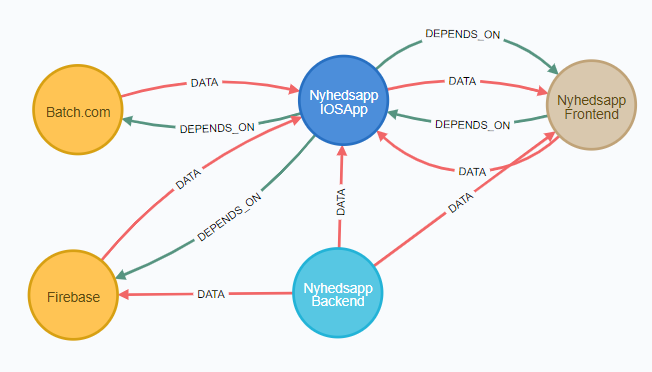
\includegraphics[width=120pt]{Nyhedsapp-IOS.PNG}
\caption{MATCH (x\{name:'Nyhedsapp IOSApp'\})- -(y) RETURN x,y}
\end{figure}
\subsubsection{Kort beskrivelse}
Afvikler Nyhedsapp-frontend, integrerer til iOS-native funktionalitet
\subsubsection{Anbefalet handling}
Nyhedsapp til både iOS og Android overholder referencearkitekturen. Der er måske ønsker om at opdatere applikationerne, så de får et mere moderne udtryk på telefonerne. Dette ønske er dog et forretningsdrevet ønske og ikke en nødvendighed set ud fra referencearkitekturen. Dette forretningsønske kan dog meget vel være med til at drive en række af de ændringer der vil være nødvendige for at programstakken under nyhedsappen bliver mere i tråd med referencearkitekturen.


\subsection{Nyhedsapp-Android}
\begin{figure}[h]
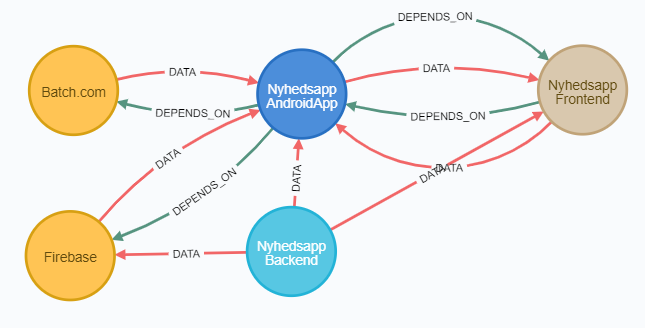
\includegraphics[width=120pt]{Nyhedsapp-Android.PNG}
\caption{MATCH (x\{name:'Nyhedsapp AndroidApp'\})- -(y) RETURN x,y}
\end{figure}
\subsubsection{Kort beskrivelse}
Native Android-wrapper, der afvikler Nyhedsapp-Frontend
\subsubsection{Anbefalet handling}
Nyhedsapp til både iOS og Android overholder referencearkitekturen. Der er måske ønsker om at opdatere applikationerne så de får et mere moderne udtryk på telefonerne. Dette ønske er dog et forretningsdrevet ønske og ikke en nødvendighed set ud fra referencearkitekturen. Dette forretningsønske kan dog meget vel være med til at drive en række af de ændringer der vil være nødvendige for at programstakken under nyhedsappen bliver mere i tråd med referencearkitekturen.


\subsection{Batch.com}
\begin{figure}[h]
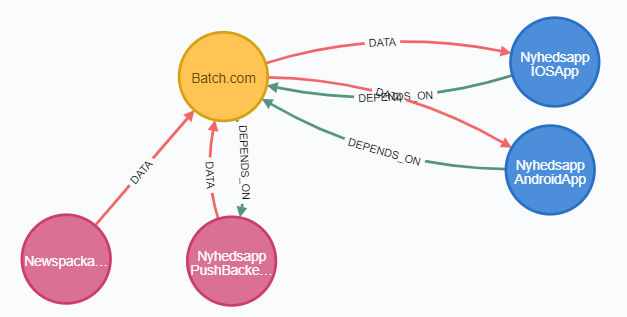
\includegraphics[width=120pt]{Batch-com.PNG}
\caption{MATCH (x\{name:'Batch.com'\})- -(y) RETURN x,y}
\end{figure}
\subsubsection{Kort beskrivelse}
SaaS tjeneste der benyttes til push af beskeder til Nyhedsapp.
Distribuerer data til Nyhedsapp-instanser, med mulighed for dublikeringskontrol så den samme enhed kun modtager data én gang, og ligeledes en opfølgningsmulighed så devices der var utilgængelige på udsendelsestidspunktet, opdateres når de er tilgængelige igen
\subsubsection{Anbefalet handling}
Tjenesten passer ind i vores referencearkitektur. Om Batch.com bliver ved med at være den bedste løsning for push af beskeder vil vi ikke tage stilling til i dette dokument.


\subsection{Firebase}
\begin{figure}[h]
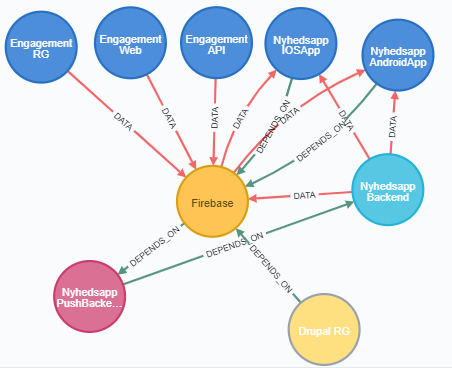
\includegraphics[width=220pt]{Firebase.PNG}
\caption{MATCH (x\{name:'Firebase'\})- -(y) RETURN x,y}
\end{figure}
\subsubsection{Kort beskrivelse}
SaaS tjeneste der benyttes til Push-service af flere applikationer:
Nyhedsapp, Drupal RG ("hvem er inde på min artikel")
% Er det virkelig tilfældet?
\subsubsection{Anbefalet handling}
Tjenesten passer ind i vores referencearkitektur. Om Firebase bliver ved med at være den bedste løsning for push af beskeder vil vi ikke tage stilling til i dette dokument.


\subsection{OCS}
\begin{figure}[h]
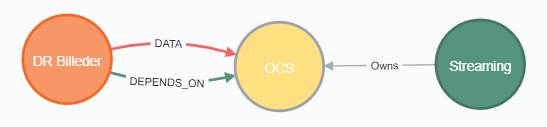
\includegraphics[width=200pt]{OCS.PNG}
\caption{MATCH (x\{name:'OCS'\})- -(y) RETURN x,y}
\end{figure}
\subsubsection{Kort beskrivelse}
API-afløseren til PSDB (MU-online), der leverer video- og radio-data (ikke anvendt i Web \& Apps endnu).

Udstiller program- og seriedata, således at aftagere kan benytte dette til at vise TV/Radio-indhold
\subsubsection{Anbefalet handling}
Ved ændringer i systemer der afhænger af PSDB, så bør det undersøges om det er relevant at anvende OCS i stedet.



\subsection{Garnnøgle}
\begin{figure}[h]
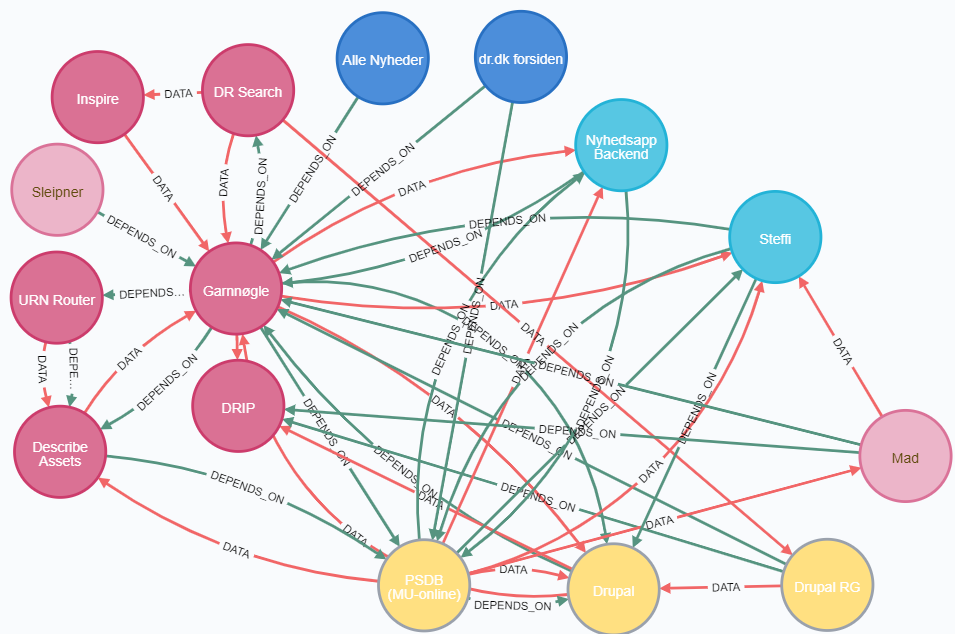
\includegraphics[width=300pt]{Garnnoegle.PNG}
\caption{MATCH (x\{name:'Garnnøgle'\})- -(y) RETURN x,y}
\end{figure}
\subsubsection{Kort beskrivelse}
Tema- og sagskategorisering af artikelindhold, således specielt nyhedsindhold kan inddeles i overordnede kategorier. Bruges også som emnebaseret abonnement-mekanisme i Nyhedsapp
Garnnøgle er ret central i værdikæden for DR.dk, da den benyttes af en lang række systemer og funktioner. Garnnøgle applikationen er behæftet med en del teknisk gæld og unødig kompleksitet i dens implementering.
\subsubsection{Anbefalet handling}
Garnnøgles placering i forhold til referencearkitekturen er ok. Selve implementeringen af garnnøgle bør dog genbesøges og afhængigt af det reelle forretningsbehov skal vi have set på en ny implementering.


\subsection{Drupal}
\begin{figure}[h]
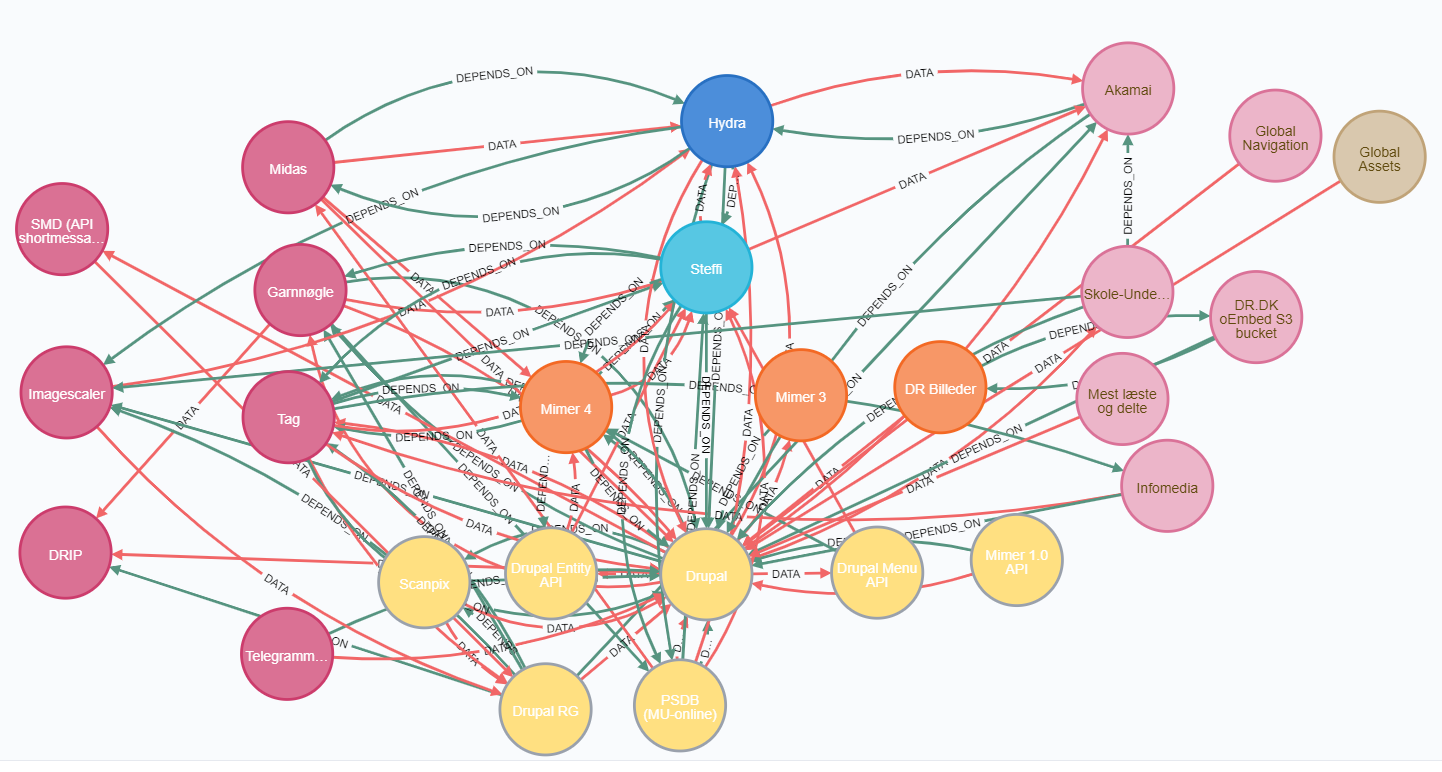
\includegraphics[width=120pt]{Drupal.PNG}
\caption{MATCH (x\{name:'Drupal'\})- -(y) RETURN x,y}
\end{figure}
\subsubsection{Kort beskrivelse}
Det primære CMS til tekstbaseret indhold på DR.dk, samt redaktionel grænseflade til indholdsproduktion og slutteligt mulighed for at grafisk opbygge sektionsforsider og sites.
\subsubsection{Anbefalet handling}
I henhold til referencearkitekturen burde Drupal kun være forbundet med Content Services og Platform Services. Da Drupal er det centrale CMS system er antallet af forbindelser ikke den store overraskelse, det peger dog entydigt på at DR stadig er meget hængt op på Drupal og dermed vil en eventuel udskiftning eller opdatering af Drupal være en stor udgift.
Vi bør helt klart se på at nedbringe antallet af direkte afhængigheder til og fra Drupal. 
Dette kan enten ske ved at lade Platform Services snakke med Content Services (f.eks. at lade garnnøgle afhænge af Mimer i stedet for Drupal), affolke og lukke de gamle udgaver af Mimer eller sikre at kun services med en god grund kan kommunikere med Drupal.

Drupal er lige nu vores styrende CMS system, det vil sige at Drupal har kontrollen med alle URL hos DR.dk, hvilket også er grunden til den direkte forbindelse fra Hydra ned til Drupal. Det vil være meget fornuftigt at kikke på at få etableret et fornuftigt URN / URL system, således at en URL / URN i sig selv er beskrivende nok til at kunne udpege det styrende indholdssystem. Det vil muliggøre sideløbende CMS systemer med hvert deres fokus og gøre det lettere at opdatere / udskifte Drupal på sigt.
 
Vi skal også have kikket på roadmap for opdatering af Drupal 7 til enten Drupal 9 eller et andet CMS system. Drupal 7 (vores nuværende installation) og efterfølgeren Drupal 8 har end of life i november 2021.
\subsubsection{Overslag}
Migrering fra Drupal 7 til andet CMS system vil være en betydelig opgave, især med det niveau af afhængigheder og egenudvikling der er foretaget på Drupal platformen. 


\subsection{Mimer 1.0 API}
\begin{figure}[h]
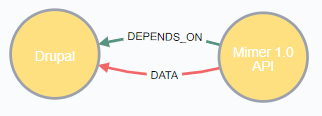
\includegraphics[width=120pt]{MimerAPI.PNG}
\caption{MATCH (x\{name:'Mimer 1.0 API'\})- -(y) RETURN x,y}
\end{figure}
\subsubsection{Kort beskrivelse}
Mimer 1.0 API er nogle REST services i Drupal, som giver Mimer 1.1 adgang til at oprette nyt indhold.
\subsubsection{Anbefalet handling}
Mimer 1.0 API er allerede under afvikling. Denne afvikling bør fortsættes og systemet lukkes.
\subsubsection{Overslag}
N/A

\subsection{Drupal RG}
\begin{figure}[h]
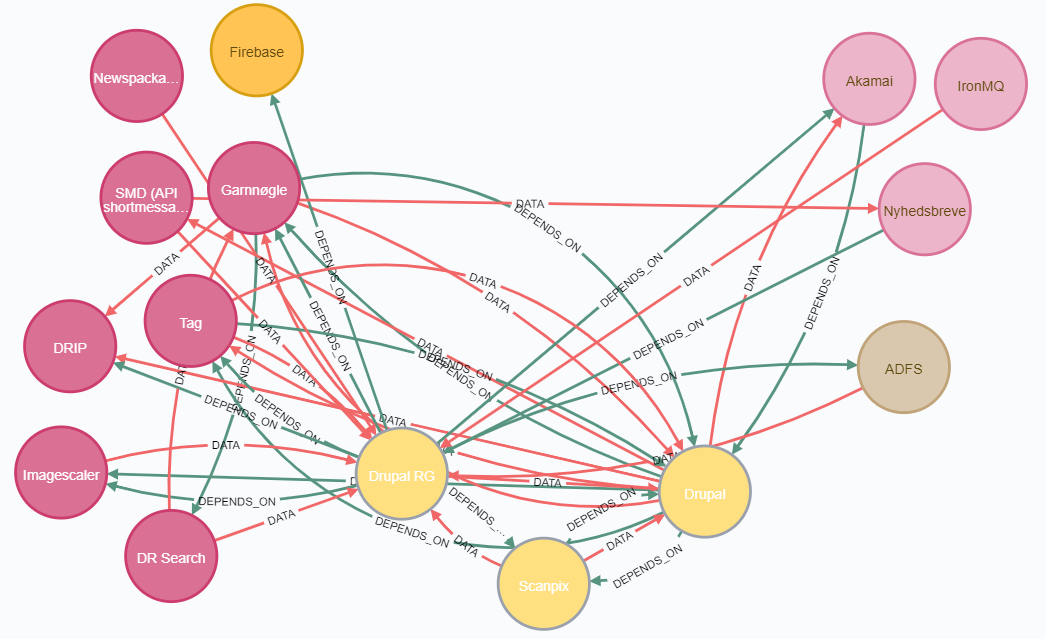
\includegraphics[width=300pt]{DrupalRG.PNG}
\caption{MATCH (x\{name:'Drupal RG'\})- -(y) RETURN x,y}
\end{figure}
\subsubsection{Kort beskrivelse}
Nyeste version af redaktør grænsefladen, lanceret Q1-2018. Redaktør grænsefladen (RG) er journalisternes værktøj til artikelproduktion. Den findes i to udgaver, hhv. RG1 og RG2.	

Webbaseret grænseflade til at oprette, redigere og distribuere tekstbaseret indhold, primært artikler. Tilbyder også integration med tema, kategoriserings, og push-funktioner.
\subsubsection{Anbefalet handling}
%TODO
\subsubsection{Overslag}


\subsection{Drupal Entity API}
\begin{figure}[h]
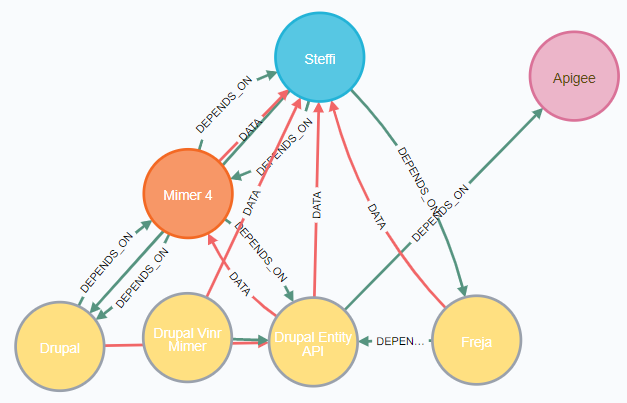
\includegraphics[width=200pt]{DrupalEntityAPI.PNG}
\caption{MATCH (x\{name:'Drupal Entity API'\})- -(y) RETURN x,y}
\end{figure}
\subsubsection{Kort beskrivelse}
Udstiller væsentlige dele af Drupals datamodel for indholdstyper i et simpelt API
\subsubsection{Anbefalet handling}
%TODO
\subsubsection{Overslag}



\subsection{Drupal Menu API}
\begin{figure}[h]
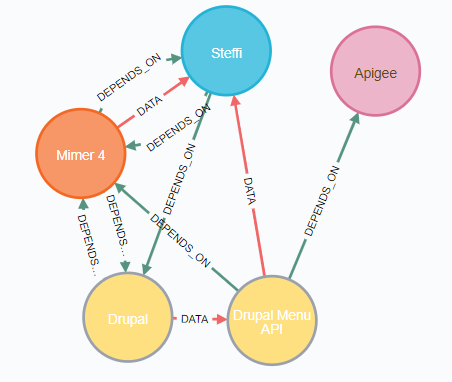
\includegraphics[width=300pt]{DrupalMenuAPI.PNG}
\caption{MATCH (x\{name:'Drupal Menu API'\})- -(y) RETURN x,y}
\end{figure}
\subsubsection{Kort beskrivelse}
Udstiller Drupals menu og sitestruktur til aftagere, der ønsker at præsentere indhold i en hierarkisk visning.
\subsubsection{Anbefalet handling}
%TODO
\subsubsection{Overslag}


\subsection{Ensighten}
\begin{figure}[h]
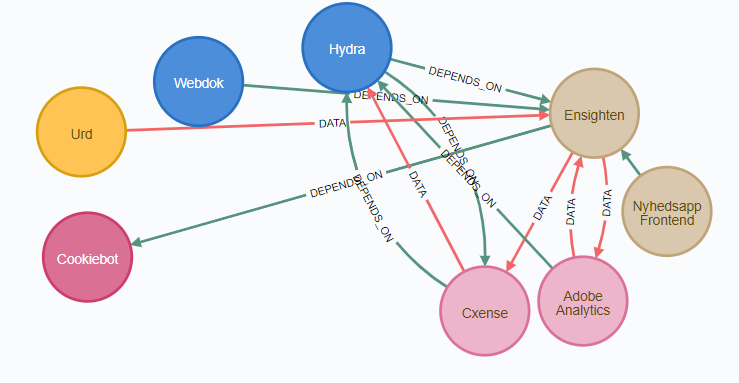
\includegraphics[width=250pt]{Ensighten.PNG}
\caption{MATCH (x\{name:'Ensighten'\})- -(y) RETURN x,y}
\end{figure}
\subsubsection{Kort beskrivelse}
Indskyder JavaScript på dr.dk sider, f.eks. til analytics, bannere, mv. Sørger derudover også for at hente og behandle metadata til analytics og anbefalingssystemer.
\subsubsection{Anbefalet handling}
\subsubsection{Overslag}


\subsection{Ad Server}
\subsubsection{Kort beskrivelse}
"Smart Ad Server" er en hosted løsning, hvor bannerhåndtering og booking/kampagner bliver håndteret. Integreres med DR applikationer der skal vise bannere til slutbrugere.
\subsubsection{Anbefalet handling}
SaaS. Der er ingen udviklingsmuligheder her, kun eventuelt at fjerne afhængigheden heraf hvis nødvendigt.
\subsubsection{Overslag}


\subsection{Midas}
\begin{figure}[h]
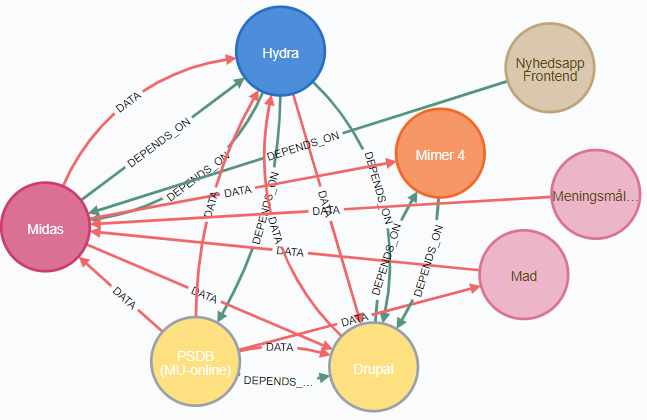
\includegraphics[width=200pt]{Midas.PNG}
\caption{MATCH (x\{name:'Midas'\})- -(y) RETURN x,y}
\end{figure}
\subsubsection{Kort beskrivelse}
Oembed-service, der omsætter oEmbed-referencer til markup, til brug i frontend.
\subsubsection{Anbefalet handling}
\subsubsection{Overslag}


\subsection{PSDB (MU-online)}
\begin{figure}[h]
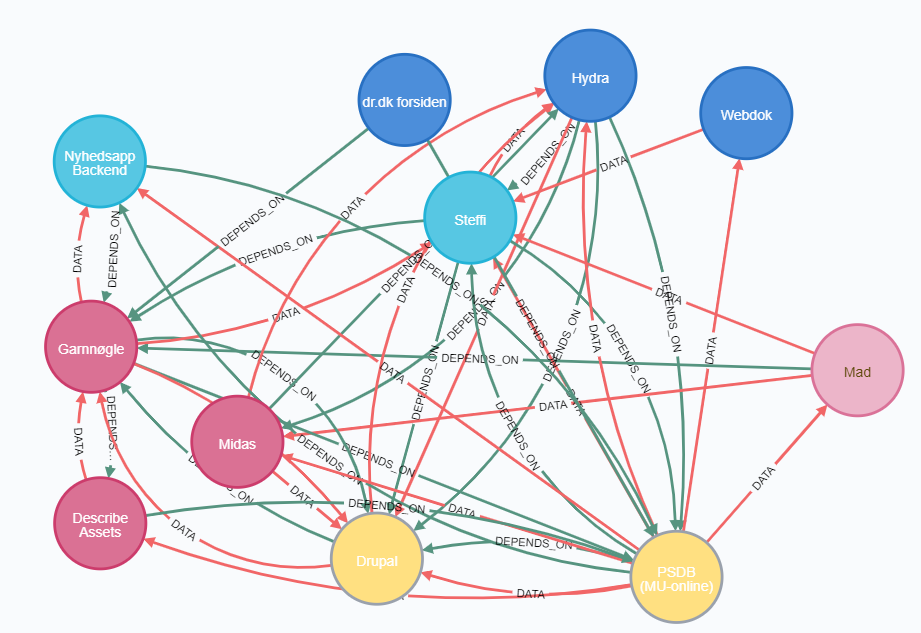
\includegraphics[width=300pt]{PSDB.PNG}
\caption{MATCH (x\{name:'PSDB (MU-online)'\})- -(y) RETURN x,y}
\end{figure}
\subsubsection{Kort beskrivelse}
Program og seriedatabase til TV-baseret indhold
\subsubsection{Anbefalet handling}
Ejerskabet af dette system ligger uden for Web og Apps.
\subsubsection{Overslag}


\subsection{Scanpix}
\begin{figure}[h]
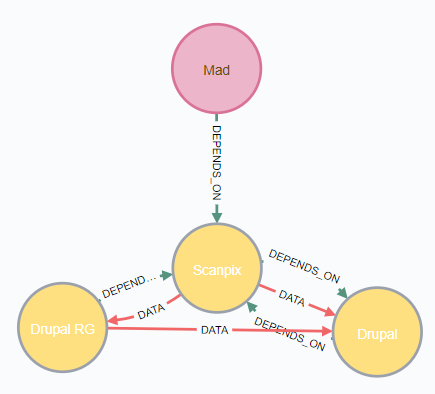
\includegraphics[width=160pt]{Scanpix.PNG}
\caption{MATCH (x\{name:'Scanpix'\})- -(y) RETURN x,y}
\end{figure}
\subsubsection{Kort beskrivelse}
Billededatabase. Ekstern service, der tilbyder redaktører at søge efter billed- og videoindhold som kan importeres og anvendes i DR's systemer.
\subsubsection{Anbefalet handling}
SaaS. Der er ingen udviklingsmuligheder her, kun eventuelt at fjerne afhængigheden heraf hvis nødvendigt.
\subsubsection{Overslag}


\subsection{Cxense}
\begin{figure}[h]
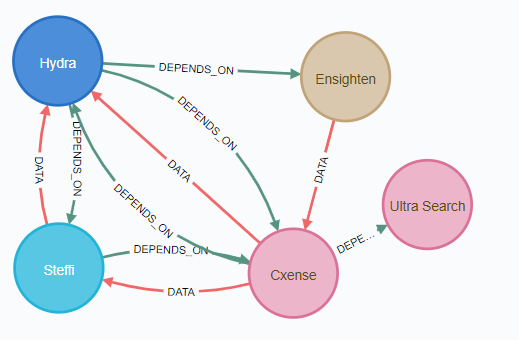
\includegraphics[width=200pt]{Cxense.PNG}
\caption{MATCH (x\{name:'Cxense'\})- -(y) RETURN x,y}
\end{figure}
\subsubsection{Kort beskrivelse}
Analysesystem til personalisering
\subsubsection{Anbefalet handling}
SaaS. Der er ingen udviklingsmuligheder her, kun eventuelt at fjerne afhængigheden heraf hvis nødvendigt.
\subsubsection{Overslag}


\subsection{Adobe Analytics}
\begin{figure}[h]
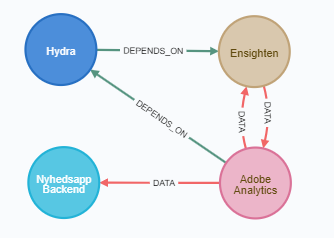
\includegraphics[width=160pt]{AdobeAnalytics.PNG}
\caption{MATCH (x\{name:'Adobe Analytics'\})- -(y) RETURN x,y}
\end{figure}
\subsubsection{Kort beskrivelse}
Analysesystem til personalisering
\subsubsection{Anbefalet handling}
SaaS. Der er ingen udviklingsmuligheder her, kun eventuelt at fjerne afhængigheden heraf hvis nødvendigt.
\subsubsection{Overslag}


\subsection{Pressebilleder}
\subsubsection{Kort beskrivelse}
Pressesite på dr.dk Udsendelse af nyhedsbreve, integration til Mosaic-billeddatabase. Sandsynligvis eksternt produkt.
\subsubsection{Anbefalet handling}
N/A
\subsubsection{Overslag}
N/A

\subsection{WebCMS}
\begin{figure}[h]
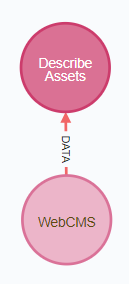
\includegraphics[height=120pt]{WebCMS.PNG}
\caption{MATCH (x\{name:'WebCMS'\})- -(y) RETURN x,y}
\end{figure}
\subsubsection{Kort beskrivelse}
Content Management System håndtering af sider på dr.dk. Udfaset og afløst af Drupal.
\subsubsection{Anbefalet handling}
N/A
\subsubsection{Overslag}
N/A

\subsection{DR Search}
\begin{figure}[h]
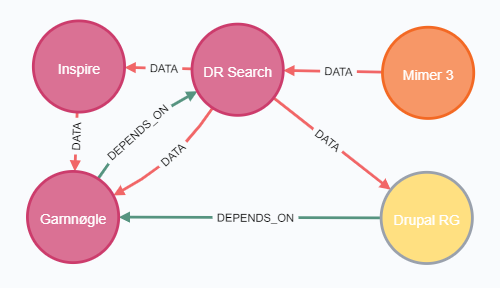
\includegraphics[width=200pt]{DRSearch.PNG}
\caption{MATCH (x\{name:'DR Search'\})- -(y) RETURN x,y}
\end{figure}
\subsubsection{Kort beskrivelse}
Søgemaskine tekst, video og radioindhold på DR.dk	

Tilbyder søgefunktionalitet med ekstrem domæneforståelse for DR's forskellige indholdstyper, distributionsregler og indholdssystemer. Kan indlejres i RG-systemer og tilbyde specialiseret søgefunktionalitet til både publiceret og ikke-publiceret indhold. Kan tilbyde slutbrugere at søge agnostisk og præsenterer søgeresultater ud fra den type indhold der er tale om, eks afspilningsoplysninger til TV-indhold. Indekserer de forskellige indholdssystemer for nyt eller opdateret indhold, og indekserer også indhold via webvisning på DR.dk
\subsubsection{Anbefalet handling}
DR Search er for tiden uden ejerskab og uden ansvarlige udviklere. Enten skal systemet adopteres af at team eller også så skal vi have afviklet systemet. Der er ikke umiddelbart et system der kan tage over som erstatning for DR Search endnu. 

%TODO 
* Skal vi erstatte?
* Skal vi beholde?
* Skal det helt skrottes?
* Kan vi benytte Drupals search til artiker, og evt streamingtjenestens søgefunktionalitet til TV / Radio?
\subsubsection{Overslag}


\subsection{Nyhedsbreve}
\begin{figure}[h]
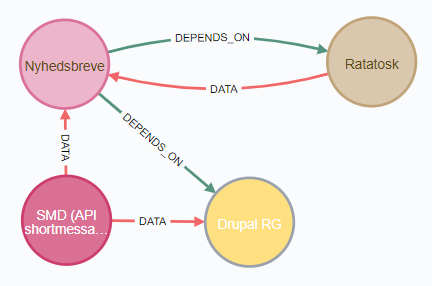
\includegraphics[width=160pt]{Nyhedsbreve.PNG}
\caption{MATCH (x\{name:'Nyhedsbreve'\})- -(y) RETURN x,y}
\end{figure}
\subsubsection{Kort beskrivelse}
Udsendelse af nyhedsbreve. Benytter Peytz' service	

Tilbyder nyhedsbreve som en distributionskanal til DR's indholdsysstemer, således at indhold kan skubbes ud til brugeren samtidig med at det publiceres på DR.dk
\subsubsection{Anbefalet handling}
SaaS men uden ejerskab. 
Det skal vurderes om denne løsning er passende for vores fremtidige arkitektur. Det er dog ikke højeste prioritet.



\subsection{DR Billeder}
\begin{figure}[h]
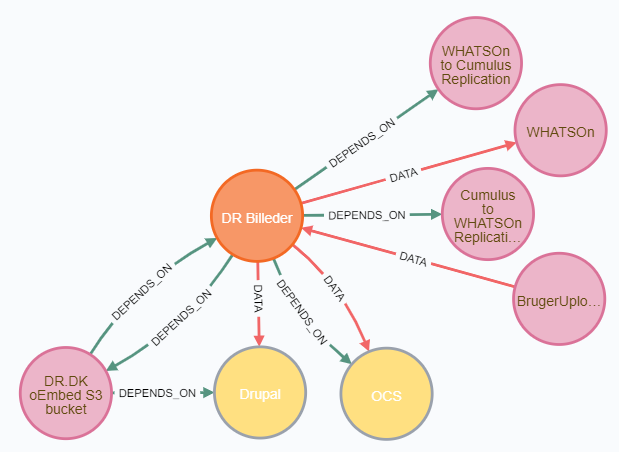
\includegraphics[width=200pt]{DRBilleder.PNG}
\caption{MATCH (x\{name:'DR Billeder'\})- -(y) RETURN x,y}
\end{figure}
\subsubsection{Kort beskrivelse}
Billedhåndteringssystem til DR's indholdsproducenter, anvender standardsystemet Cumulus fra Canto. Der anvendes en underleverandør, Attention, til at konfigurere systemet. Består af følgende delkomponenter: Database, applikationsserver, web UI, tyk klient.
\subsubsection{Anbefalet handling}
Ingen handling nødvendig. Systemet håndteres uden for Web og Apps



\subsection{DR.DK oEmbed S3 bucket}
\begin{figure}[h]
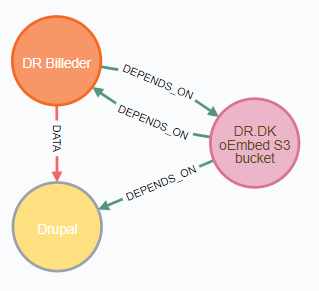
\includegraphics[width=120pt]{S3Bucket.PNG}
\caption{MATCH (x\{name:'DR.DK oEmbed S3 bucket'\})- -(y) RETURN x,y}
\end{figure}
\subsubsection{Kort beskrivelse}
En AWS S3 bucket der anvendes til online versioner af billeder som indlejres med oEmbed
\subsubsection{Anbefalet handling}
Ingen handling nødvendig. Systemet håndteres uden for Web og Apps



\subsection{Mimer 3}
\begin{figure}[h]
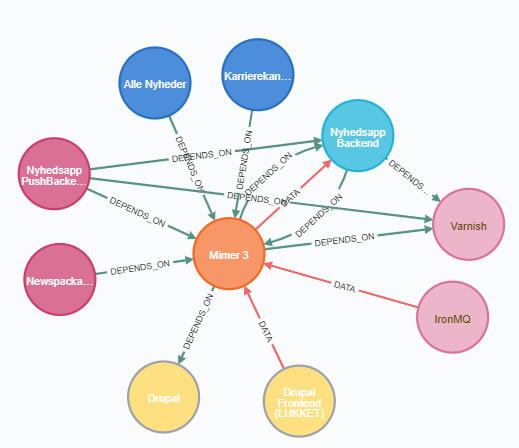
\includegraphics[width=300pt]{Mimer3.PNG}
\caption{MATCH (x\{name:'Mimer 3'\})- -(y) RETURN x,y}
\end{figure}
\subsubsection{Kort beskrivelse}
API til Drupals artikelindhold.

Udstiller Drupals primære indholdstyper til brug og visning i andre systemer.
\subsubsection{Anbefalet handling}
Mimer 3 er under afvikling. Det viste billede af afhængigheder er stadig ved at skrumpe. Mimer 3 bør afvikles helt og fjernes, så vi slipper for at have parallelle implementeringer der løser de samme opgaver.
\subsubsection{Overslag}
Der mangler stadig mange afhængigheder der skal migreres over på Mimer 4. Disse er dog i pipeline.


\subsection{Mimer 4}
\begin{figure}[h]
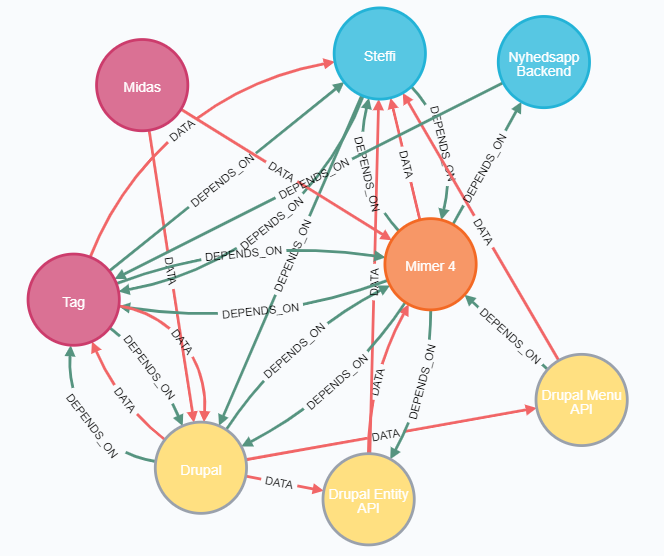
\includegraphics[width=200pt]{Mimer4.PNG}
\caption{MATCH (x\{name:'Mimer 4'\})- -(y) RETURN x,y}
\end{figure}
\subsubsection{Kort beskrivelse}
API til Drupals artikelindhold.

Udstiller Drupals primære indholdstyper til brug og visning i andre systemer.
\subsubsection{Anbefalet handling}



\subsection{Tag}
\begin{figure}[h]
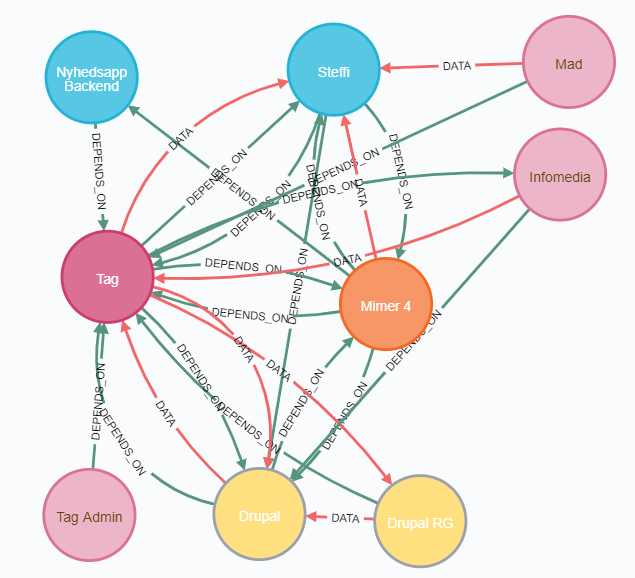
\includegraphics[width=200pt]{Tag.PNG}
\caption{MATCH (x\{name:'Tag'\})- -(y) RETURN x,y}
\end{figure}
\subsubsection{Kort beskrivelse}
Tagsystem til opmærkning af DR's web-indhold.
\subsubsection{Anbefalet handling}
Tag manager systemet bliver slet ikke brugt i det omfang det burde. Sidste opdatering er fra marts 2018. Vi bør sammen med opdateringen af garnnøgle se på om vi kan enten bygge Tag systemet sammen med Garnnøgles erstatning eller helt udskifte Tag systemet til noget der stemmer mere overens med de behov vi har.



\subsection{Urd}
\begin{figure}[h]
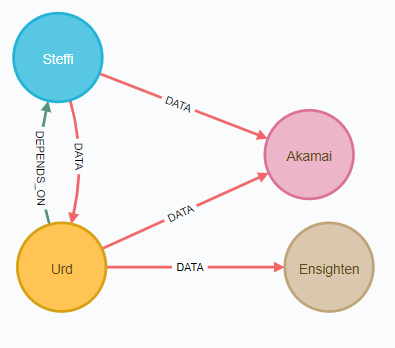
\includegraphics[width=160pt]{Urd.PNG}
\caption{MATCH (x\{name:'Urd'\})- -(y) RETURN x,y}
\end{figure}
\subsubsection{Kort beskrivelse}
Metadataservice, der leverer metadata til brug i TMS
\subsubsection{Anbefalet handling}



\subsection{Infomedia}
\begin{figure}[h]
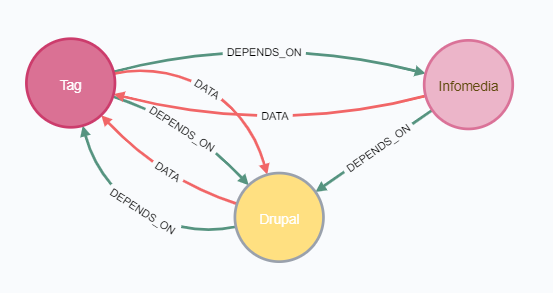
\includegraphics[width=130pt]{Infomedia.PNG}
\caption{MATCH (x\{name:'Infomedia'\})- -(y) RETURN x,y}
\end{figure}
\subsubsection{Kort beskrivelse}
Taksonomidatabase og tekstanalysesystem til tags.

Tilbyder en komplet, vedligeholdt taksonomi samt tekstanalysefunktionalitet, der kan analysere en given tekst og indikere tags fra taksonomien som er relevante.

\subsubsection{Anbefalet handling}
Infomedia bruges idag til tag systemet. Tag systemet og Garnnøgle står formentligt over for en større omskrivning. Om Infomedia skal benyttes til tekstanalyse og forslag til Tagging af artikler skal vi have set nærmere på.



\subsection{Auth0}
\begin{figure}[h]
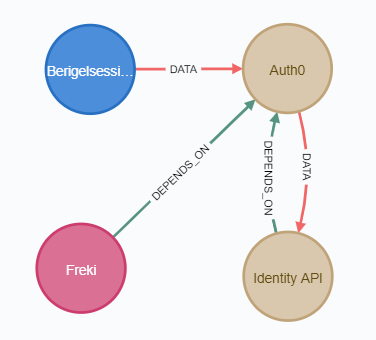
\includegraphics[width=130pt]{Auth0.PNG}
\caption{MATCH (x\{name:'Auth0'\})- -(y) RETURN x,y}
\end{figure}
\subsubsection{Kort beskrivelse}
Oauth autentifikations platform. SaaS.
\subsubsection{Anbefalet handling}
Auth0 er en fin platform til autentificering af brugere. Det er en betalt service, der passer godt ind i vores eksisterende programstak. 



\subsection{Identity API}
\begin{figure}[h]
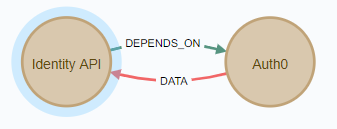
\includegraphics[width=130pt]{Identity.PNG}
\caption{MATCH (x\{name:'Identity API'\})- -(y) RETURN x,y}
\end{figure}
\subsubsection{Kort beskrivelse}
Backend til DR's login-løsning.
\subsubsection{Anbefalet handling}
Ingen nødvendig


\subsection{Telegrammaskine}
\begin{figure}[h]
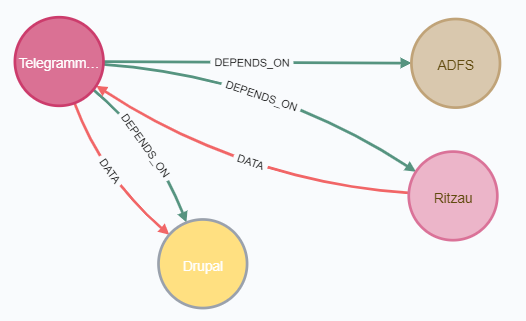
\includegraphics[width=200pt]{Telegrammaskine.PNG}
\caption{MATCH (x\{name:'Telegrammaskine'\})- -(y) RETURN x,y}
\end{figure}
\subsubsection{Kort beskrivelse}
Integration til Ritzau-indhold, med mulighed for at redigere og udgive telegrammer som Drupal-artikler.	

DR modtager løbende nyhedsunderretninger fra Ritzau i form af telegrammer; Telegrammaskinen tilbyder redaktører en meget hurtig måde at overskue seneste telegrammer samt at publicere disse direkte på DR.dk
\subsubsection{Anbefalet handling}
Ingen ændringer nødvendigt.


\subsection{Dr. Edition}
\begin{figure}[h]
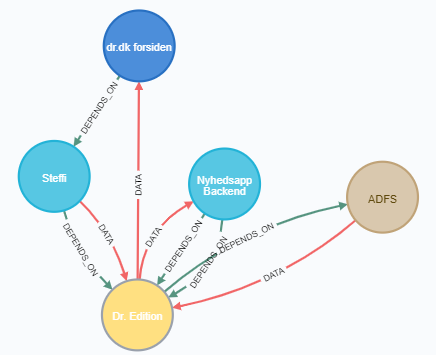
\includegraphics[width=220pt]{DrEdition.PNG}
\caption{MATCH (x\{name:'Dr. Edition'\})- -(y) RETURN x,y}
\end{figure}
\subsubsection{Kort beskrivelse}
Forsideværktøj til forsiden af DR.dk, hvor redaktører udarbejder forsider, inkluderer også API. Benytter Aptomas Dr. Edition-produkt. (steffi kommer snart til at trække til den nye forside). 

Tilbyder forsideredaktører at opbygge og redigere forsiden af DR.dk ud fra seneste udgivne artikelindhold fra Drupal, samt at versionere og skifte mellem flere forskellige forsideudgaver.
\subsubsection{Anbefalet handling}



\subsection{dr.dk forsiden}
\begin{figure}[h]
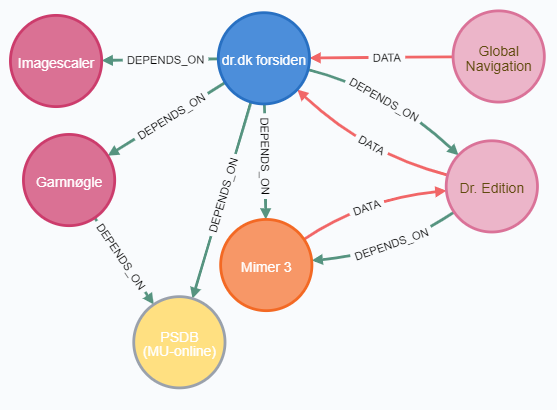
\includegraphics[width=160pt]{DrDkForsiden.PNG}
\caption{MATCH (x\{name:'dr.dk forsiden'\})- -(y) RETURN x,y}
\end{figure}
\subsubsection{Kort beskrivelse}
Azure-driftet ASP.NET MVC applikation til at hente data og vise forsiden af dr.dk

Robust system til visning af de forsider som forsideredaktører udarbejder i Dr. Edition.
\subsubsection{Anbefalet handling}



\subsection{Alle Nyheder}
\begin{figure}[h]
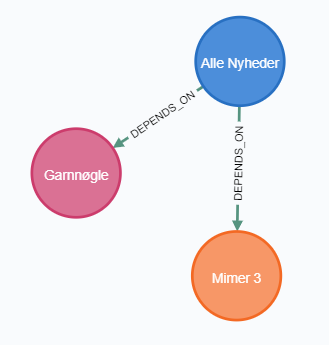
\includegraphics[width=120pt]{AlleNyheder.PNG}
\caption{MATCH (x\{name:'Alle Nyheder'\})- -(y) RETURN x,y}
\end{figure}
\subsubsection{Kort beskrivelse}
Systemet der driver siden allenyheder (alle nyheder): http://www.dr.dk/nyheder/allenyheder/	

Tilbyder overblik over senest publiceret artikelindhold samt en søgning ud fra publiceringstidspunkt
\subsubsection{Anbefalet handling}



\subsection{Newsapp UI}
\begin{figure}[h]
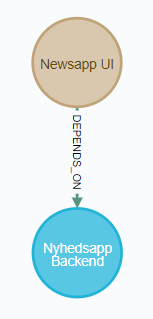
\includegraphics[width=50pt]{NyhedsAppUi.PNG}
\caption{MATCH (x\{name:'Newsapp UI'\})- -(y) RETURN x,y}
\end{figure}
\subsubsection{Kort beskrivelse}
Web-renderingsværktøj til DR Nyheder (app). Web-hostet værktøj til at se mobil app i web-version. Placeret på https://www.dr.dk/tjenester/newsapp-ui/.	

Redaktørvendt visning af hvordan indhold vises i Nyhedsapp, således at redaktører kan lave Nyhedsapp-specifikt preview af indhold.
\subsubsection{Anbefalet handling}
Ingen nødvendig. Applikationen lever eller dør med de 2 nyheds App


\subsection{SMD (API shortmessage-dispatcher)}
\begin{figure}[h]
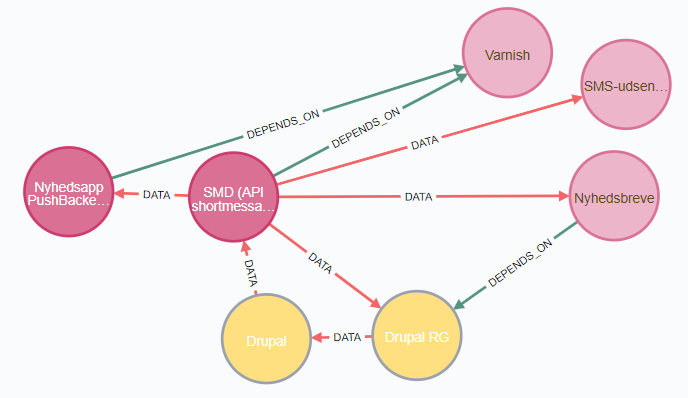
\includegraphics[width=120pt]{SMD.PNG}
\caption{MATCH (x\{name:'SMD (API shortmessage-dispatcher)'\})- -(y) RETURN x,y}
\end{figure}
\subsubsection{Kort beskrivelse}
Push SMS; nyhedsbrev, Nyheds app. fra f.eks. Drupal, facebook.

Tilbyder push af tekstbaseret indhold til en række forskellige platforme og distributionsmekanismer
\subsubsection{Anbefalet handling}



\subsection{Mest læste og delte}
\begin{figure}[h]
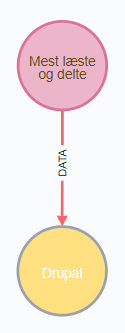
\includegraphics[height=120pt]{MestL.PNG}
\caption{MATCH (x\{name:'Mest læste og delte'\})- -(y) RETURN x,y}
\end{figure}
\subsubsection{Kort beskrivelse}
ESI mest læste og delte mm. på DR.dk og Drupal sider.

Tilbyder en liste af mest besøgt og delt (via social medier) indhold ud fra besøgsstatistik.
\subsubsection{Anbefalet handling}
Applikationen skal lukkes ned, da dens funktionalitet bliver erstattet af Cxense.



\subsection{Nyhedsapp Backend}
\begin{figure}[h]
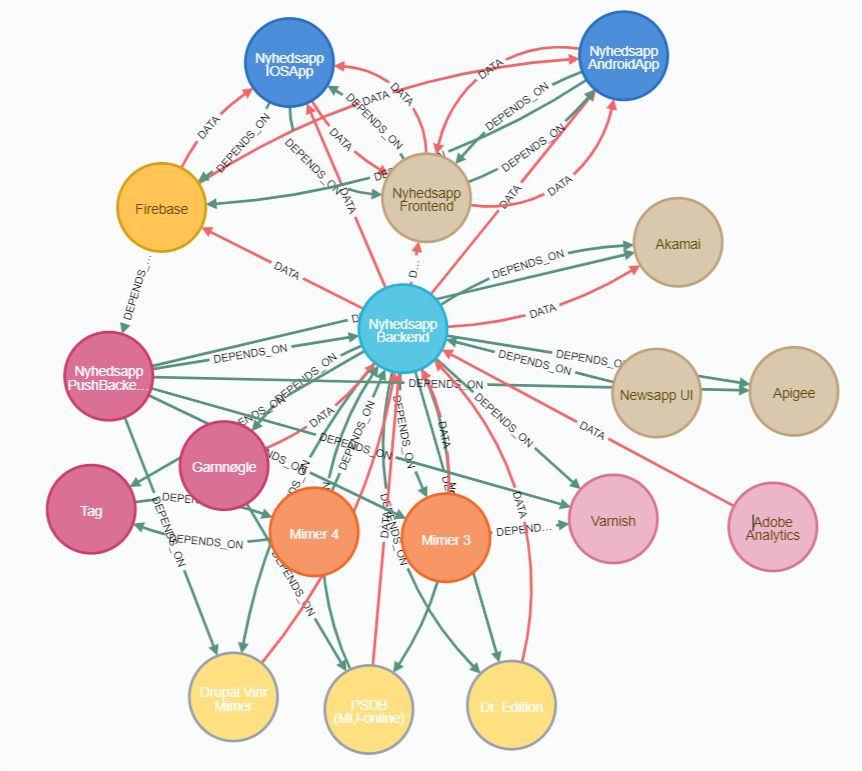
\includegraphics[height=200pt]{NyhedsappBE.PNG}
\caption{MATCH (x\{name:'Nyhedsapp Backend'\})- -(y) RETURN x,y}
\end{figure}
\subsubsection{Kort beskrivelse}
Backend til DR's Nyhedsapp.	

Applikation der indsamler, aggregerer og transformerer artikler til DRs nyhedsapps dataformat. Persisterer og udstiller data for Nyhedsapp (Nyhedsapp Frontend).
\subsubsection{Anbefalet handling}
Nyhedsapp Backend forekommer også som en parallel implementering af funktionalitet der allerede eksisterer andet steds i DR.dk. 
Artikeldata burde blive udstillet igennem Steffi på lige fod med hjemmesiden og Nyhedsapp backend burde kun varetage funktionaliteten der adskiller Nyhedsapp fra hjemmesiden. Det vil sige push beskeder, brugerstyrring, abonnementer og lignende. 
\subsubsection{Overslag}
Det virker ikke rationelt at omskrive nyhedsapp kun med henblik på at rydde lidt op i systemlandskabet, men når vi på et tidspunkt skal genbesøge nyhedsapp med henblik på modernisering bør vi også sikre at vi følger den anbefalede arkitektur og dermed indhenter content i veldefineret format fra den fælles content aggregation service.

\subsection{Tag Admin}
\begin{figure}[h]
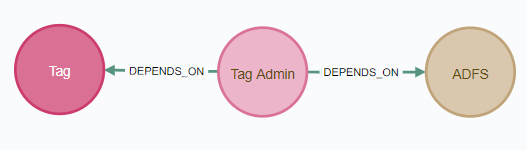
\includegraphics[width=120pt]{TagAdmin.PNG}
\caption{MATCH (x\{name:'Tag Admin'\})- -(y) RETURN x,y}
\end{figure}
\subsubsection{Kort beskrivelse}
Administrative interface for Tag API.
Rent frontend produkt der er integreret som en del af Drupal
\subsubsection{Anbefalet handling}
Tag API skal vi have kikket på i den generelle renovation af Relations systemer.
\subsubsection{Overslag}


\subsection{Ritzau}
\begin{figure}[h]
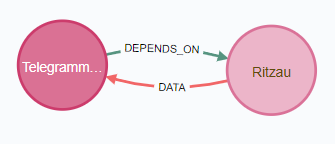
\includegraphics[width=80pt]{Ritzau.PNG}
\caption{MATCH (x\{name:'Ritzau'\})- -(y) RETURN x,y}
\end{figure}
\subsubsection{Kort beskrivelse}
Eksternt system. Dataleverandør til Drupal-artikler.
Tilbyder bred dækning af nyhedsbilledet i form af kortfattede telegrammer.
\subsubsection{Anbefalet handling}
Eksternt system som er kritisk for redaktionen. Ingen handling nødvendig.



\subsection{Ratatosk}
\begin{figure}[h]
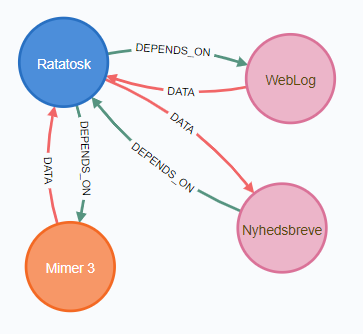
\includegraphics[width=80pt]{Ratatosk.PNG}
\caption{MATCH (x\{name:'Ratatosk'\})- -(y) RETURN x,y}
\end{figure}
\subsubsection{Kort beskrivelse}
RSS feed generator. Leverer data til Nyhedsbreve.


\subsection{Drupal Vinr Mimer}
\begin{figure}[h]
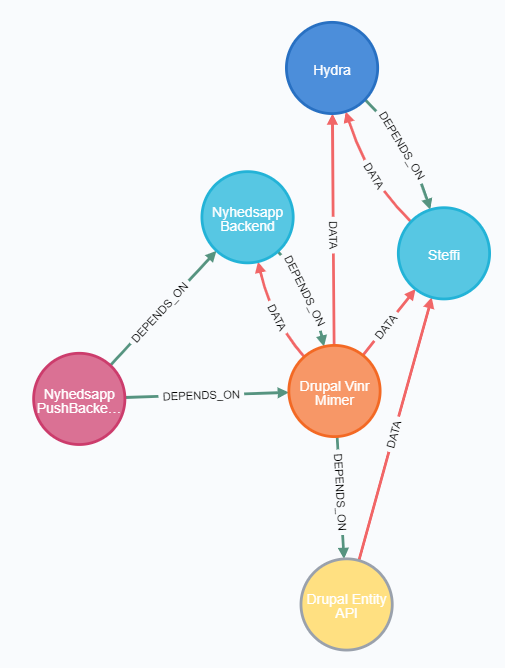
\includegraphics[width=120pt]{DrupalVinrMimer.PNG}
\caption{MATCH (x\{name:'Drupal Vinr Mimer'\})- -(y) RETURN x,y}
\end{figure}
\subsubsection{Kort beskrivelse}
Mikroservice til at udstille indhold ud fra flere forskellige identifikationsmuligheder
\subsubsection{Anbefalet handling}
I forbindelse med alignment med reference arkitekturen, så skal vi have kikket på om denne service har et eksistensgrundlag eller om den skal erstattes af en anden.


\subsection{DRIP}
\begin{figure}[h]
\includegraphics[width=120pt]{DRIP.PNG}
\caption{MATCH (x\{name:'DRIP'\})- -(y) RETURN x,y}
\end{figure}
\subsubsection{Kort beskrivelse}
DR Integrationsplatform, et køsystem til udveksling og transformation af beskeder mellem systemer. Har ind- og ud-adapters.
Tilbyder applikationer at udveksle data pålideligt samt at distribuere til mange forskellige aftagere.
\subsubsection{Anbefalet handling}
Systemet ejes af Virksomhedssystemer, så vil ikke være oplagt at ændre på ud fra ønsker i Web \& Apps. 
Skal muligvis erstattes af et Event system alt efter hvad analysen af det viser.


\subsection{Global Navigation}
\begin{figure}[h]
\includegraphics[width=120pt]{GlobalNavigation.PNG}
\caption{MATCH (x\{name:'Global Navigation'\})- -(y) RETURN x,y}
\end{figure}
\subsubsection{Kort beskrivelse}
Global top navigation og footer.
Script der indsætter navigation og footer på dr.dk.
\subsubsection{Anbefalet handling}
Ingen umiddelbart nødvendig.


\subsection{BrugerUpload}
\begin{figure}[h]
\includegraphics[width=80pt]{BrugerUpload.PNG}
\caption{MATCH (x\{name:'BrugerUpload'\})- -(y) RETURN x,y}
\end{figure}
\subsubsection{Kort beskrivelse}
React komponent med egen backend, der bl.a. bruges til upload af brugernes egne vejrbilleder. Har sin egen Drupal komponent.
\subsubsection{Anbefalet handling}
Ingen umiddelbart nødvendig.


\subsection{Imagescaler}
\begin{figure}[h]
\includegraphics[width=160pt]{Imagescaler.PNG}
\caption{MATCH (x\{name:'Imagescaler'\})- -(y) RETURN x,y}
\end{figure}
\subsubsection{Kort beskrivelse}
Egenudviklet billedskaleringsservice, som Drupal RG og frontend anvender til at skalere billeder efter behov.	

Billedskalering, konvertering og systemspecifikke workarounds for at aftage billeder.
\subsubsection{Anbefalet handling}
Der er ingen udestående problemer med Imagescaler som den står nu. 


\subsection{ADFS}
\begin{figure}[h]
\includegraphics[width=120pt]{ADFS.PNG}
\caption{MATCH (x\{name:'ADFS'\})- -(y) RETURN x,y}
\end{figure}
\subsubsection{Kort beskrivelse}
Active Directory Federation Service, SSO for DR-brugere.

SSO-loginservice til DR's ansatte, så de kan anvende samme login til alle systemer.
\subsubsection{Anbefalet handling}
Der er ingen udeståender problemer med ADFS som den står nu.


\subsection{Global Assets}
\begin{figure}[h]
\includegraphics[width=80pt]{GlobalAssets.PNG}
\caption{MATCH (x\{name:'Global Assets'\})- -(y) RETURN x,y}
\end{figure}
\subsubsection{Kort beskrivelse}
Globale JavaScript og CSS assets, primært til gammelt dr.dk design.
\subsubsection{Anbefalet handling}
Da Global Assets primært benyttes af det gamle design, så virker det oplagt at vi kikker på om det giver mening at bibeholde de gamle sider. Det kan meget vel give mening at få ryddet lidt op og her kunne være et oplagt sted at starte.


\subsection{Global}
\begin{figure}[h]
\includegraphics[width=80pt]{Global.PNG}
\caption{MATCH (x\{name:'Global'\})- -(y) RETURN x,y}
\end{figure}
\subsubsection{Kort beskrivelse}
Globale front-end assets (JS, CSS, fonte), mere strømlinet erstatning for Global Assets. Hostes på Heroku.
\subsubsection{Anbefalet handling}
Der er ingen udeståender problemer med Global som den står nu.


\subsection{Webstat}
\begin{figure}[h]
\includegraphics[width=60pt]{Webstat.PNG}
\caption{MATCH (x\{name:'Webstat'\})- -(y) RETURN x,y}
\end{figure}
\subsubsection{Kort beskrivelse}
Diverse statistik (mv.) scripts. Det meste af funktionaliteten håndteres i dag af Ensighten men f.eks. Gallup håndteres stadig af Webstat.
\subsubsection{Anbefalet handling}
I oprydningens ånd, så skal vi have kikket på om det er relevant at få Webstat pensioneret og de sidste anvendere flyttet til f.eks. Ensighten.


\subsection{Describe Assets}
\begin{figure}[h]
\includegraphics[width=120pt]{DescribeAssets.PNG}
\caption{MATCH (x\{name:'Describe Assets'\})- -(y) RETURN x,y}
\end{figure}
\subsubsection{Kort beskrivelse}
Udstiller data for givne indholdsressourcer (tre separate services for hvert større indholdssystem).

Ud fra en URN kan Describe Assets udstille de relevante data for denne URN, som en hurtig og endpoint-agnostisk service der omsætter et ID til data
\subsubsection{Anbefalet handling}
Der er ingen udeståender problemer med Describe Assets som den står nu. Når vi kikker nærmere på vores generelle Datamodel og URN / URL, så kan det meget vel være der også kommer opgaver til Describe Assets.


\subsection{URN Router}
\begin{figure}[h]
\includegraphics[width=80pt]{URNRouter.PNG}
\caption{MATCH (x\{name:'URN Router'\})- -(y) RETURN x,y}
\end{figure}
\subsubsection{Kort beskrivelse}
URN-oversætter, der returnerer links til Describe Assets.

For at afskærme aftagere fra hvilke systemer der udstiller hvilke typer indhold, tilbyder URN Router ét samlet endpoint hvortil en URN kan sendes, og der returneres en URL til et endpoint hvor de ønskede data om den givne URN kan hentes.
\subsubsection{Anbefalet handling}
Der er ingen udeståender problemer med URN Router som den står nu. Når vi kikker nærmere på vores generelle Datamodel og URN / URL, så kan det meget vel være der også kommer opgaver til URN Router.


\subsection{Freja}
\begin{figure}[h]
\includegraphics[width=80pt]{Freja.PNG}
\caption{MATCH (x\{name:'CHANGE'\})- -(y) RETURN x,y}
\end{figure}
\subsubsection{Kort beskrivelse}
Drupal 8 site, præsentation og forside API.	

RG samt API til vedligeholdelse og udstilling af præsentationsdata vedr. Drupal sektioner, forsider og artikelsider, f.eks. farver, logoer, backdrops.
\subsubsection{Anbefalet handling}
Der er ingen udeståender problemer med Freja som den står nu.


\subsection{Karrierekanonen}
\begin{figure}[h]
\includegraphics[width=60pt]{Karrierekanonen.PNG}
\caption{MATCH (x\{name:'Karrierekanonen'\})- -(y) RETURN x,y}
\end{figure}
\subsubsection{Kort beskrivelse}
Applikation til musik, præsentation (Front-end + admin)
\subsubsection{Anbefalet handling}
Der er ingen udeståender problemer med Karrierekanonen som den står nu.


\subsection{Apigee}
\begin{figure}[h]
\includegraphics[width=120pt]{Apigee.PNG}
\caption{MATCH (x\{name:'Apigee'\})- -(y) RETURN x,y}
\end{figure}
\subsubsection{Kort beskrivelse}
API-gateway for DR's backendsystemer hostet udenfor DR Byen.

API-gateway, der afskærmer backendsystemer fra DDoS-angreb, tilbyder API-authentication og nøglehåndtering.
\subsubsection{Anbefalet handling}
Det giver rigtigt god mening at alle de APIer vi udstiller ligger bag en god API-gateway. Vi skal have kikket på præcist hvad vi gør med API gateway når vi begynder at nærme os at flytte systemer over på pipeline


\subsection{Varnish}
\begin{figure}[h]
\includegraphics[width=160pt]{Varnish.PNG}
\caption{MATCH (x\{name:'Varnish'\})- -(y) RETURN x,y}
\end{figure}
\subsubsection{Kort beskrivelse}
Håndterer caching og routing, primært for systemer hostet i DR Byen.

Varnish sikrer at forespørgsler til backends eller andre services rammer et centralt sted, og derefter sendes til den relevante service eller backend, samt tilbyder cachingmuligheder for svaret, således at belastningen på service eller backend reduceres kraftigt.
\subsubsection{Anbefalet handling}
Varnish er i sig selv ikke noget vi kan påvirke i Web \& Apps. Vores afhængighed af systemet hænger sammen med afhængigheden af de systemer der ligger bag Varnish. 
De systemer der benytter Varnish i dag er enten nogen der allerede er planer for at erstatte eller ligger i systemer som vi ikke kan påvirke.


\subsection{Freki}
\begin{figure}[h]
\includegraphics[width=80pt]{Freki.PNG}
\caption{MATCH (x\{name:'Freki'\})- -(y) RETURN x,y}
\end{figure}
\subsubsection{Kort beskrivelse}
System til at gemme applikations specifik personfølsom data.
\subsubsection{Anbefalet handling}
Der er ingen udeståender problemer med Freki som den står nu.



\subsection{Berigelsessider}
\begin{figure}[h]
\includegraphics[width=80pt]{Berigelsessider.PNG}
\caption{MATCH (x\{name:'Berigelsessider'\})- -(y) RETURN x,y}
\end{figure}
\subsubsection{Kort beskrivelse}
Opsamler ekstra data om en bruger i forbindelse med Login.
\subsubsection{Anbefalet handling}
Der er ingen udeståender problemer med Berigelsessider som den står nu.



\subsection{IronMQ}
\begin{figure}[h]
\includegraphics[width=80pt]{IronMQ.PNG}
\caption{MATCH (x\{name:'IronMQ'\})- -(y) RETURN x,y}
\end{figure}
\subsubsection{Kort beskrivelse}
Køsystem til tilstandsløs integration mellem systemer, primært udenfor DR Byen.

Varetager modtagelse og distribution af beskeder mellem systemer, kan underrette aftagende systemer når der er nyt indhold i en given kø, fremfor at disse systemer poller IronMQ.

SaaS implementering, så dermed ikke noget vi kan udvikle på selv.
\subsubsection{Anbefalet handling}
En eventbaseret tilgang til opdatering af systemer er i mange tilfælde en strålende løsning og gerne også en vi skal have kikket nærmere på. Om vi skal benytte IronMQ eller et andet pub / sub system skal vi have kikket nærmere på.


\end{document}
